\documentclass[12pt]{article}
\usepackage[english]{babel}
\usepackage{natbib}
\usepackage{url}
\usepackage[utf8x]{inputenc}
\usepackage{amsmath}
\usepackage{graphicx}
\graphicspath{{images/}}
\usepackage{parskip}
\usepackage{fancyhdr}
\usepackage{vmargin}
\setmarginsrb{3 cm}{2.5 cm}{3 cm}{2.5 cm}{1 cm}{1.5 cm}{1 cm}{1.5 cm}


\documentclass{article}
\usepackage[svgnames]{xcolor}
\usepackage{listings}

\lstset{language=R,
    basicstyle=\small\ttfamily,
    stringstyle=\color{DarkGreen},
    otherkeywords={0,1,2,3,4,5,6,7,8,9},
    morekeywords={TRUE,FALSE},
    deletekeywords={data,frame,length,as,character},
    keywordstyle=\color{blue},
    commentstyle=\color{DarkGreen},
}



\title{lab Assignment 8}								% Title
\author{Ocampo}								% Author
\date{12 Sept 2015}											% Date

\makeatletter
\let\thetitle\@title
\let\theauthor\@author
\let\thedate\@date
\makeatother

\pagestyle{fancy}
\fancyhf{}
\rhead{\theauthor}
\lhead{\thetitle}
\cfoot{\thepage}

\begin{document}

%%%%%%%%%%%%%%%%%%%%%%%%%%%%%%%%%%%%%%%%%%%%%%%%%%%%%%%%%%%%%%%%%%%%%%%%%%%%%%%%%%%%%%%%%

\begin{titlepage}
	\centering
    \vspace*{0.5 cm}
    
\includegraphics[scale = 0.75]{pictures.png}\\[1.0 cm]	% University Logo
    	% University Name
				% Course Code
	\rule{\linewidth}{0.2 mm} \\[0.4 cm]
	{ \huge \bfseries \thetitle}\\
	\rule{\linewidth}{0.2 mm} \\[1.5 cm]
	
	\begin{minipage}{0.4\textwidth}
		\begin{flushleft} \large
			\emph{Submitted To:}\\
			CMPSC 390\\
             Prof. Oliver Bonham-Carter\\
            
			\end{flushleft}
			\end{minipage}~
			\begin{minipage}{0.4\textwidth}
            
			\begin{flushright} \large
			\emph{Submitted By :} \\
			Daniel Ocampo\\
 
            Fall Semester  \\
		\end{flushright}
		
	
        
	\end{minipage}\\[2 cm]
	
	
\end{titlepage}

%%%%%%%%%%%%%%%%%%%%%%%%%%%%%%%%%%%%%%%%%%%%%%%%%%%%%%%%%%%%%%%%%%%%%%%%%%%%%%%%%%%%%%%%%

\tableofcontents
\pagebreak

%%%%%%%%%%%%%%%%%%%%%%%%%%%%%%%%%%%%%%%%%%%%%%%%%%%%%%%%%%%%%%%%%%%%%%%%%%%%%%%%%%%%%%%%%

\section{Objective}

To explore statistical tools which are relevant for the evaluation of economic data. At this point in
the class, there has already been much exposure to using many different types of statistical tools to
handle different formats of data. It is therefore expected that the student will able to research code
development and will be able to resolve data formatting issues during while working in the analysis
of data. In particular, these skills comprise the ability to research R-statistics software packages for
the application to the particular contexts for which they were designed and to extract knowledge
from the produced visualizations and extracted interpretation of results. Furthermore, the student
will be able to explain credible results and conclusions which are to be entirely supported by the
methods and data.




  
\section{Reading assignment}
In the article by Heathcote et al. [1], female labor supply is discussed for its impact on the United
States economy between the years of 1967 to 2002. The authors produce a model which was designed
to help study and measure the below factors which are associated to women in the workforce.

Our data originates from [2] and concerns the lifestyles, living conditions and economic contri-
butions made by women on the world’s stage between the years of 1960 to 2017. In this lab, you
are to use this data to gather direct or indirect proof to either support or refute the claims made
by the four themed questions (listed above) of the study by Heathcote et al.
For each of its four themes, determine the necessary variables from the data set in the spread-
sheet which could be used to support or refute the claims of the article. Remember, the exact
questions from the article may not be directly answerable by simply running tests over the in-
cluded data, and so you will have to develop a strategy in which you will use the correlations of
several variables, or multi-linear models to argue your point. For this step, your selected variables will amass proof that could be used to describe scenarios or conditions which will support or refute
the conclusions of the authors.


\subsection{The Article’s Themed Questions}


\begin{enumerate}
\item The decline in marriage rates,
\item The narrowing gender wage gap,
\item  The preference (or cultural) shift towards market work, and
\item  The change in womens bargaining power within the household.
\end{enumerate}
\section{ R code that was Used}


\begin{lstlisting}

library(gapminder)
library(dplyr)
library(tidyverse)
library(ggplot2)
library(psych)

library(ctv)
twoCountry <- read.csv(file = "/home/o/ocampod/fall2017/cs390-ochampoo/Data-Analytics/Lab8/lab8Data.csv", header=TRUE, sep= ",")
View(twoCountry)
twoCountry[1,]

###### Question 1 ######The decline in marriage rates,

WifeBeater <- filter(
  twoCountry ,
  Indicator.Name ==  "Women who believe a husband is justified in beating his wife (any of five reasons) (%)"
  )

View(WifeBeater)

WifeBeater <- filter(
  WifeBeater, Country.Name == "Peru" | Country.Name == "Senegal")### Countries with the most data

write.csv(WifeBeater, file = "/home/o/ocampod/fall2017/cs390-ochampoo/Data-Analytics/Lab8/Data/wifeBeater.csv")

WifeBeater <- read.csv(file = "/home/o/ocampod/fall2017/cs390-ochampoo/Data-Analytics/Lab8/Data/wifeBeaterLiner.csv", header=TRUE, sep= ",")


qplot(Peru, unmarried, data = WifeBeater, alpha = I(1/4)) + geom_smooth(method = lm, se = F)
qplot(Senegal, unmarried, data = WifeBeater, alpha = I(1/4)) + geom_smooth(method = lm, se = F)
View(WifeBeater)
### we can see that that less women are less likely to let their husband beat the m 

LiteracyGender <- filter(#### this going to say if women are getting more educated, therefore make more money for themselves 
  twoCountry,
  Indicator.Name ==  "Literacy rate, adult female (% of females ages 15 and above)"
)

View(LiteracyGender)


LiteracyGender <- filter(#### this going to say if women are getting more educated, therefore make more money for themselves 
  LiteracyGender,
  Country.Name ==  "Spain" | Country.Name ==  "Turkey" 
)

write.csv(LiteracyGender, file = "/home/o/ocampod/fall2017/cs390-ochampoo/Data-Analytics/Lab8/Data/LiteracyRate.csv")


LiteracyGender <- read.csv(file = "/home/o/ocampod/fall2017/cs390-ochampoo/Data-Analytics/Lab8/Data/LiteracyRateLiner.csv", header=TRUE, sep= ",")

qplot(Spain, unmarried, data = LiteracyGender, alpha = I(1/4)) + geom_smooth(method = lm, se = F)
qplot(Turkey, unmarried, data = LiteracyGender, alpha = I(1/4)) + geom_smooth(method = lm, se = F)
View(LiteracyGender)



####################################### End Of Question 1 #################

############## Question 2 ############# The narrowing gender wage gap,
schooling <- filter(
  twoCountry ,
  Indicator.Name ==  "Expected years of schooling, female" 
  
  )

schooling <- filter(
  schooling ,
  Country.Name ==  "Finland" | Country.Name ==  "Greece"
  )

write.csv(schooling, file = "/home/o/ocampod/fall2017/cs390-ochampoo/Data-Analytics/Lab8/Data/schooling.csv")


schooling <- read.csv(file = "/home/o/ocampod/fall2017/cs390-ochampoo/Data-Analytics/Lab8/Data/schoolingCor.csv", header=TRUE, sep= ",")
Finland <- select(schooling,Finland,Q1)
cor(Finland,method = "pearson")
Greece <- select(schooling,Greece,Q1)
cor(Finland)
pairs.panels(Finland)
pairs.panels(Greece)
describe(schooling)
corPlot(Greece)
View(schooling)

####################### end of  Question 2  #############



### Question 3 ###### preference (or cultural) shift towards market work


laborforceGender <- filter(
  twoCountry ,
  Indicator.Name ==  "Labor force, female")


laborforceGender <- filter(
  laborforceGender ,  
  Country.Name  ==  "Mexico" | Country.Name  ==  "United States"
)

write.csv(laborforceGender, file = "/home/o/ocampod/fall2017/cs390-ochampoo/Data-Analytics/Lab8/Data/laborforceGender.csv")



laborforceGender <- read.csv(file = "/home/o/ocampod/fall2017/cs390-ochampoo/Data-Analytics/Lab8/Data/laborforceGendergraph.csv", header=TRUE, sep= ",")  

test <- select(laborforceGender,MEX,Year)
View(test)
t.test(test)

laborforceGender[1,]

qplot(MEX, Year, data = laborforceGender, alpha = I(1/4)) + geom_smooth(method = lm, se = F)



laborforceGender %>% ggplot(aes(x = MEX, y = Year)) +
  geom_point(alpha = I(1/4)) + geom_smooth()


View(laborforceGender)


















##### End of question 3 ##########
#### Question 4 ### The change in womens bargaining power within the household.

homeowners <- filter(
  twoCountry ,
  Indicator.Name ==  "Women who own a house alone (\% of women age 15-49)"
)
View(homeowners)
#### was not able to obtain enough data for this one but most of the data showed that most country had little female house ownership 
### A house 

decisionMaker <- filter(
  twoCountry ,
 Indicator.Name ==  "Decision maker about a woman's own health care: mainly wife (\% of women age 15-49)"
)
View(decisionMaker)

write.csv(decisionMaker, file = "/home/o/ocampod/fall2017/cs390-ochampoo/Data-Analytics/Lab8/Data/decisionMaker.csv")


decisionMaker <- filter(
  decisionMaker ,
  Country.Name ==  "Peru" | Country.Name ==  "Bangladesh"
)

write.csv(decisionMaker, file = "/home/o/ocampod/fall2017/cs390-ochampoo/Data-Analytics/Lab8/Data/decisionMaker.csv")

decisionMakerGraph <- read.csv(file = "/home/o/ocampod/fall2017/cs390-ochampoo/Data-Analytics/Lab8/Data/decisionMakerGraph.csv", header=TRUE, sep= ",")

summary(decisionMakerGraph)



decisionMakerGraph \%>\% ggplot(aes(x = Peru, y = Year)) +
  geom_point(alpha = I(1/4)) + geom_smooth()

decisionMakerGraph \%>\% ggplot(aes(x = Bangladesh, y = Year)) +
  geom_point(alpha = I(1/4)) + geom_smooth()




View(decisionMakerGraph)


major<- filter(
   twoCountry,
  Indicator.Name ==  "Decision maker about major household purchases: mainly husband (\% of women age 15-49)" 
  )

major<- filter(
  major,
  Country.Name ==  "Peru" 
)

write.csv(major, file = "/home/o/ocampod/fall2017/cs390-ochampoo/Data-Analytics/Lab8/Data/major.csv")

major <- read.csv(file = "/home/o/ocampod/fall2017/cs390-ochampoo/Data-Analytics/Lab8/Data/MarjorGraph.csv", header=TRUE, sep= ",")
ggplot(data = major) +
  geom_point(mapping = aes(x = Year, y = PER))
t.test(major)
View(major)


major \%>\% ggplot(aes(x = PER, y = Year)) +
  geom_point(alpha = I(1/4)) + geom_smooth()



###########End of question 4####


### Intresting Data 

womenHiv <- filter(
  twoCountry,
  Indicator.Name ==  "Women's share of population ages 15+ living with HIV (%)"
)


employ <- filter(
  twoCountry ,
  Indicator.Name ==  "Employment to population ratio, 15+, female (\%) (modeled ILO estimate)
" | Indicator.Name ==  "Employment to population ratio, 15+, male (\%) (modeled ILO estimate)
"
)


married <- filter(
  twoCountry ,
  Indicator.Name ==  "Women who were first married by age 18 (\% of women ages 20-24)"
)


SavedForEducation <- filter(
  twoCountry ,
  Indicator.Name ==  "Saved for education or school fees, female (\% age 15+) [w2]" | Indicator.Name ==  "Literacy rate, adult male (\% of males ages 15 and above)
")

View(SavedForEducation)

laborforceGender <- filter(
  twoCountry ,
  Indicator.Name ==  "Labor force, female")

View(laborforceGender)

femaleWage <- filter(
  twoCountry ,
  Indicator.Name ==  "Wage and salaried workers, female (\% of female employment)" | Indicator.Name ==  "Wage and salaried workers, male (\% of male employment)"
)

Childemploy <- filter(
  twoCountry ,
  Indicator.Name ==  "Children in employment, female (\% of female children ages 7-14)" | Indicator.Name ==  "Children in employment, male (\% of male children ages 7-14)
"
)


business <- filter(
  twoCountry ,
  Indicator.Name ==  "Cost of business start-up procedures, female (\% of GNI per capita)
" | Indicator.Name ==  "Cost of business start-up procedures, male (\% of GNI per capita)"
)



View(twoCountry)









\end{lstlisting}



 

\section{Personal Idea}


The way we answered this question was by filtering the data 
From The world Bank Gender statistics. After filtering I was able to pick up data by manually looking at the data. I was considering using the like method but , the dataset was small enough to look at. 


\begin{enumerate}
\item The decline in marriage rates,

The filter that was used to support or reject this theory was "Women who believe a husband is justified in beating his wife (any of five reasons) (\%)". I chose the both Peru and Senegal, the reason I chose both of these country was because they had the most of data. Even then I had to manipulate the data so that it can fit. So for example I would to take the average of two data point so that I can get the middle missing data. In \textbf{figure 1} and In \textbf{figure 2} we see that women are less likely to think it is okay to beat women. 


The Next data set that we chose was "Literacy rate, adult female (\% of females ages 15 and above)." The reason I chose this data set was because of the simple fact that more educated would have a higher chance to have a job, and thus be more independent. In \textbf{Figure 3} We have a dataset  



\item The narrowing gender wage gap



For this dataset I look for country with most amount of data, which it happened to be Finland and Greece. These two countries had most data on the topic of, "Expected years of schooling, female". well the data shows that the more educated women get the more she will make.  











\item  The preference (or cultural) shift towards market work

This one was women in the labor force, I feel that it more and more common to see women working instead of being a stay at home mom. there is more and more women joing the work force both in the US and Mexico. 


\item  The change in womens bargaining power within the household.

This one is a little difficult to answer because of the simple fact that there was nearly no data. But with that data I did find I was able to conclude that women did not have may not have much of a bargaining power.\\

I came to the conclusion based on my data of  "Decision maker about a woman's own health care: mainly wife (\% of women age 15-49)" For peru, there was a little spike in women who had less of say about their own health.  While also Bangladesh there were little spikes but still increasing. \\


The next one which was also difficult to answer because of lack of data was "Decision maker about major household purchases: mainly husband (\% of women age 15-49)"
The only country that enough data was Peru, and we can see that it had it ups and downs when it came making decision. ultimately based the correlation graph women were having a say.  


\end{enumerate}

\section{Statement 1: The decline in marriage rates}

\begin{figure}[h]
\caption{The decline in marriage rates in peru:"Decision maker about major household purchases: mainly husband (\% of women age 15-49)"}
\centering
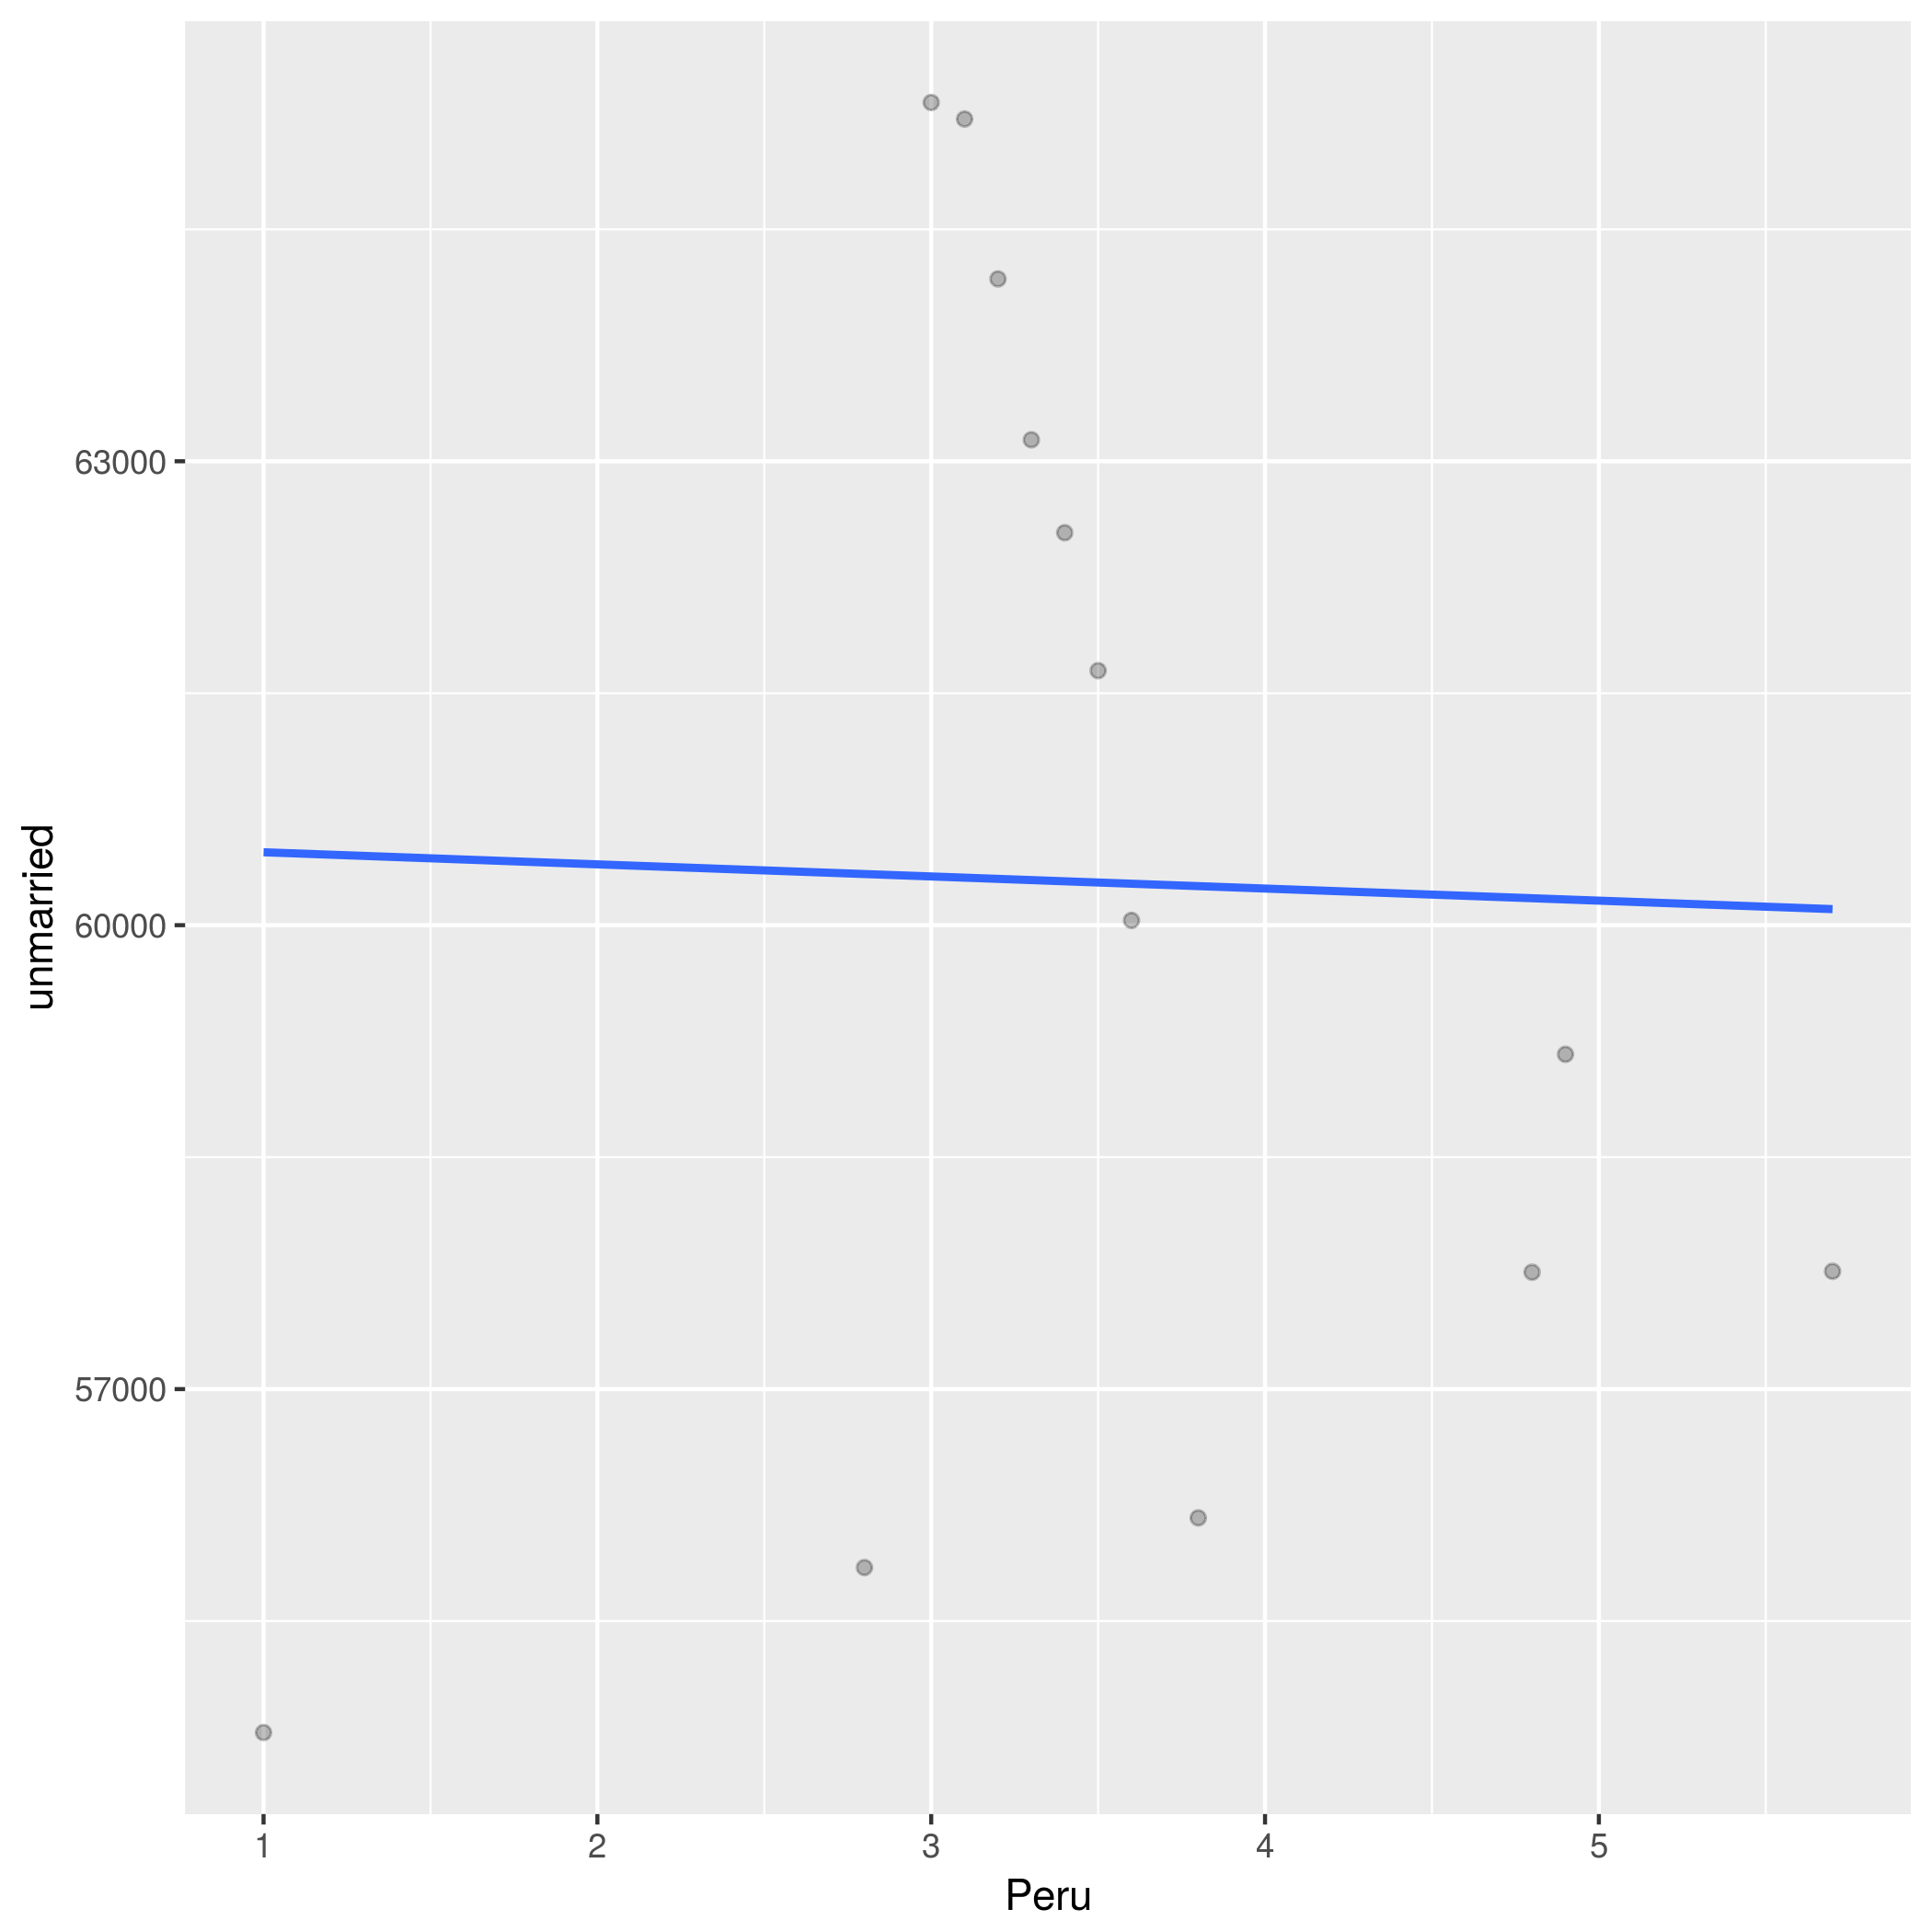
\includegraphics[scale=.5]{quest1Peru.png}
\end{figure}
 \clearpage
\begin{figure}[h!]
\caption{The decline in marriage rates in Senegal:"Decision maker about major household purchases: mainly husband (\% of women age 15-49)"}
\centering
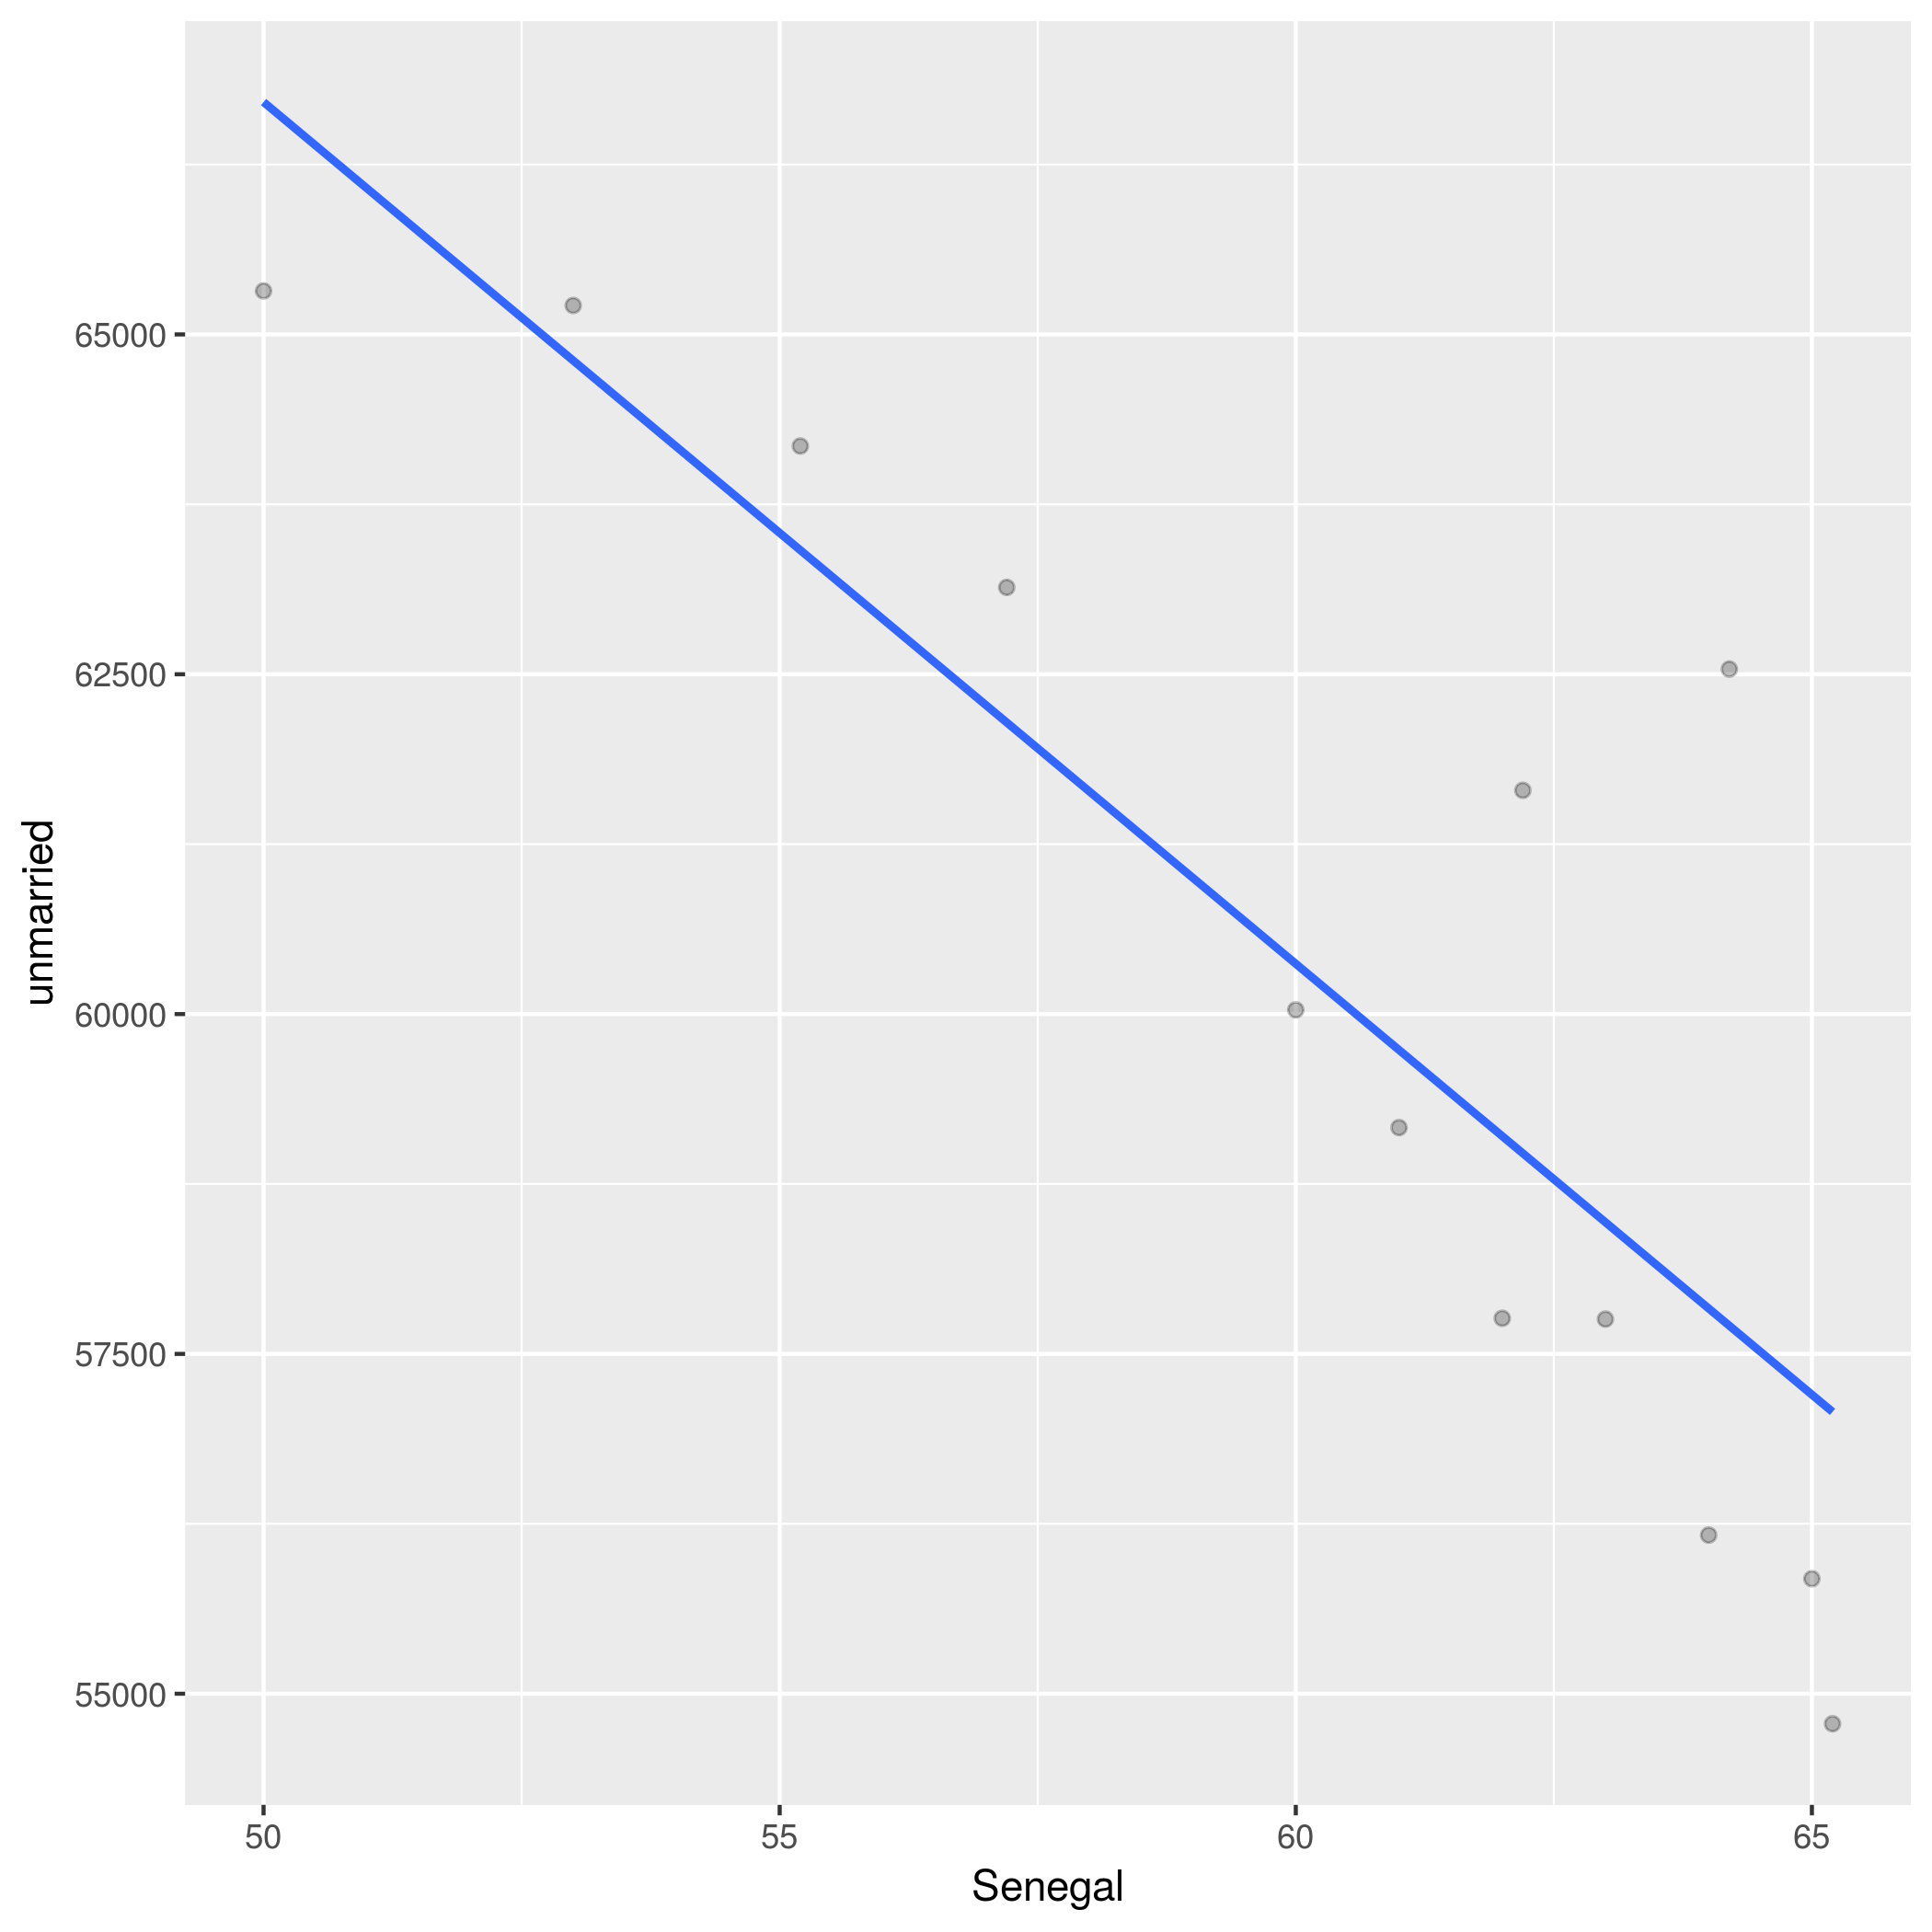
\includegraphics[scale=.5]{quest1Senegal.png}
\end{figure}
 \clearpage

\begin{figure}[h!]
\caption{The decline in marriage rates in Senegal}
\centering
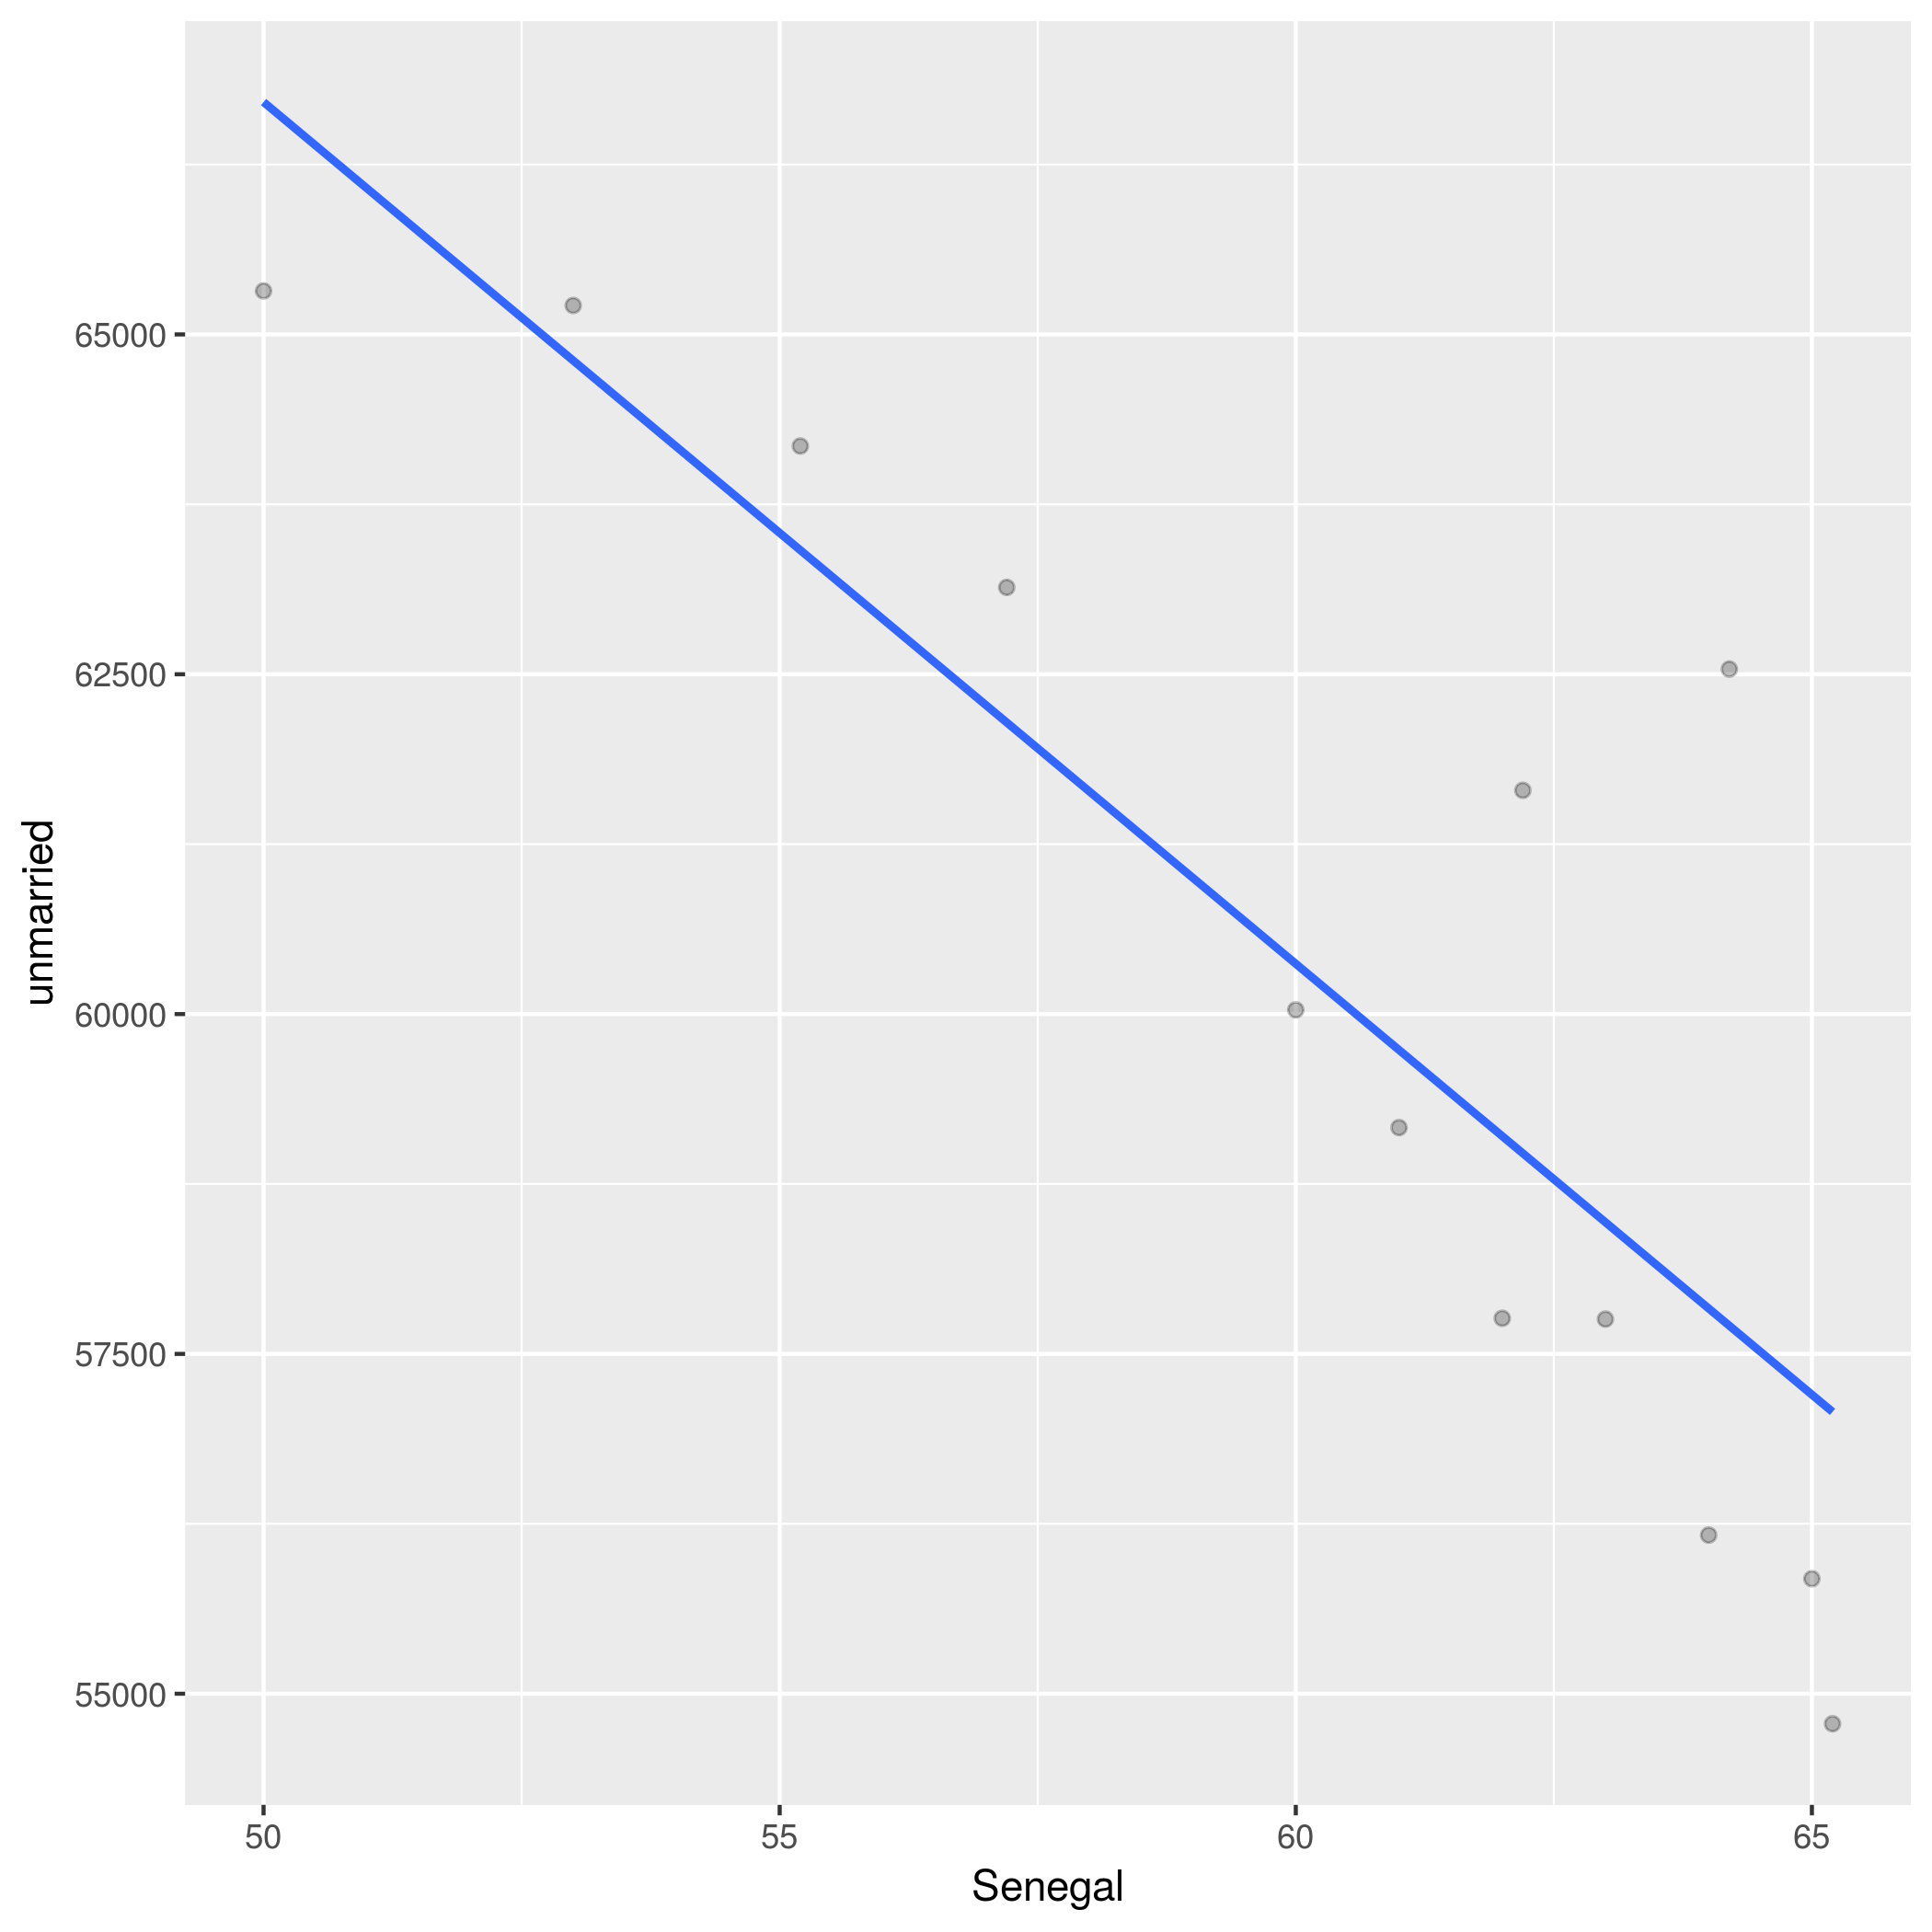
\includegraphics[scale=.5]{quest1Senegal.png}
\end{figure}
 \clearpage

\begin{figure}[h!]
\caption{The decline in marriage rates in Turkey}
\centering
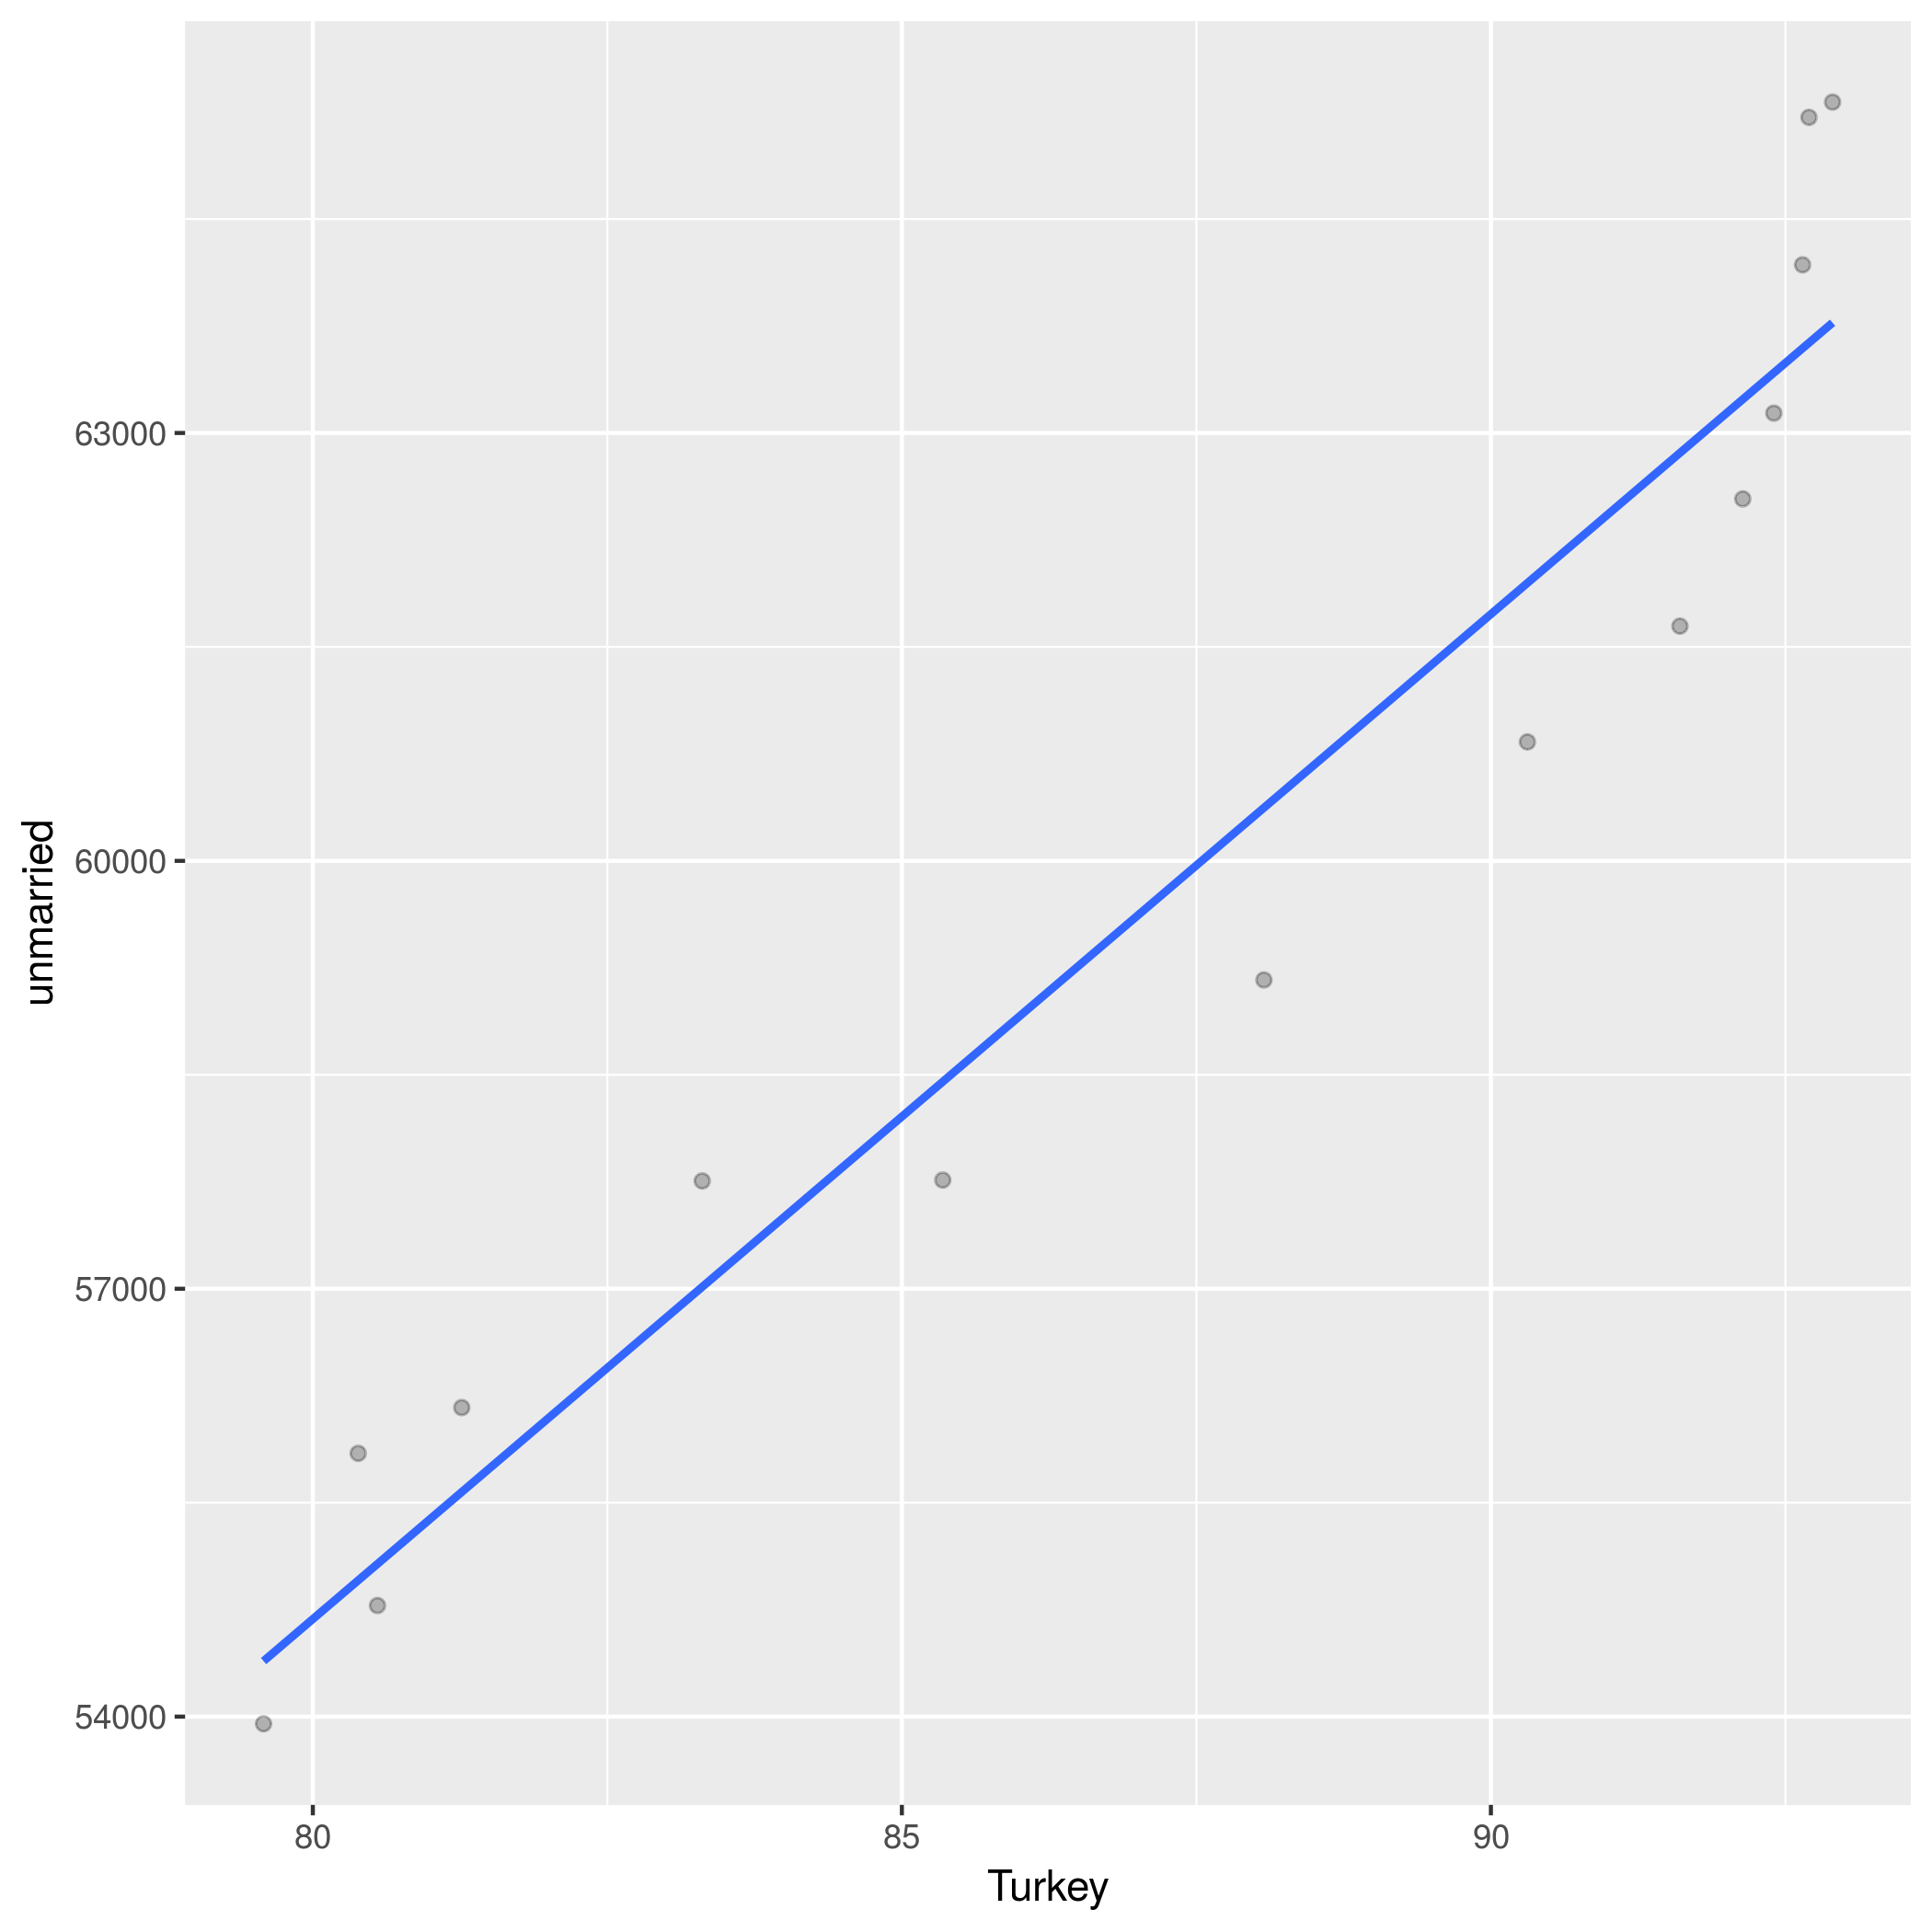
\includegraphics[scale=.5]{quest1Turkey.png}
\end{figure}
 \clearpage



\section{Statement 2:The narrowing gender wage gap}

\begin{figure}[h!]
\caption{Increase of women going to school for Finland, and earning more as the years progress}
\centering
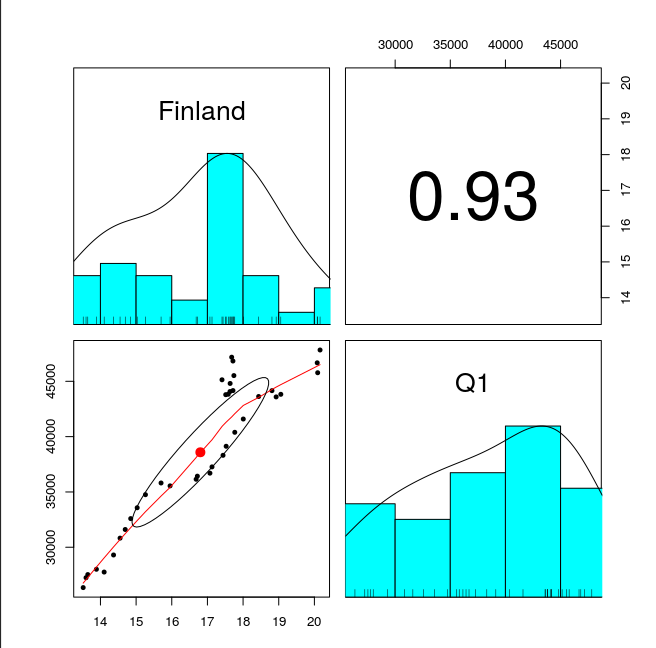
\includegraphics[scale=.5]{quest2Finland.png}
\end{figure}
\clearpage

\begin{figure}[h!]
\caption{Increase in women going to school  with an increase in pay Greece}
\centering
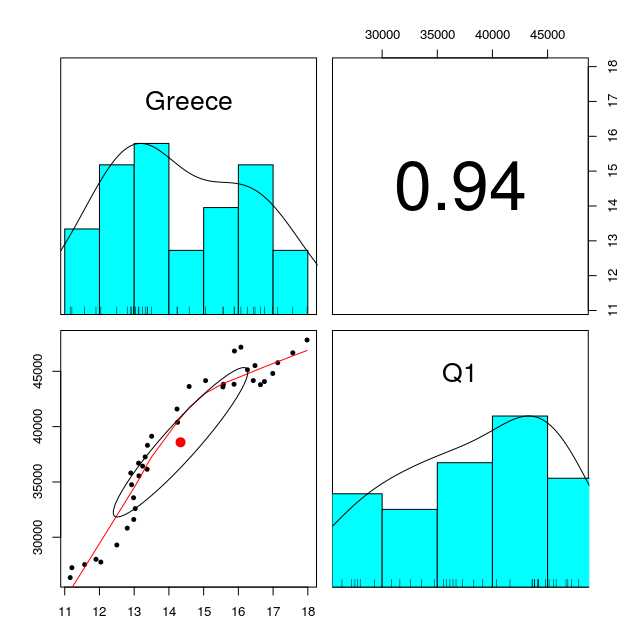
\includegraphics[scale=.5]{quest2Greece.png}
\end{figure}

\begin{figure}[h!]
\caption{T test example}
\centering
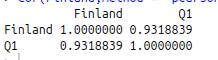
\includegraphics[scale=.5]{questFinlandCor.png}
\end{figure}

\clearpage


\section{Statement 3: The preference (or cultural) shift towards market work }

\begin{figure}[h!]
\caption{Increase of women in the Labor force for Mexico  }
\centering
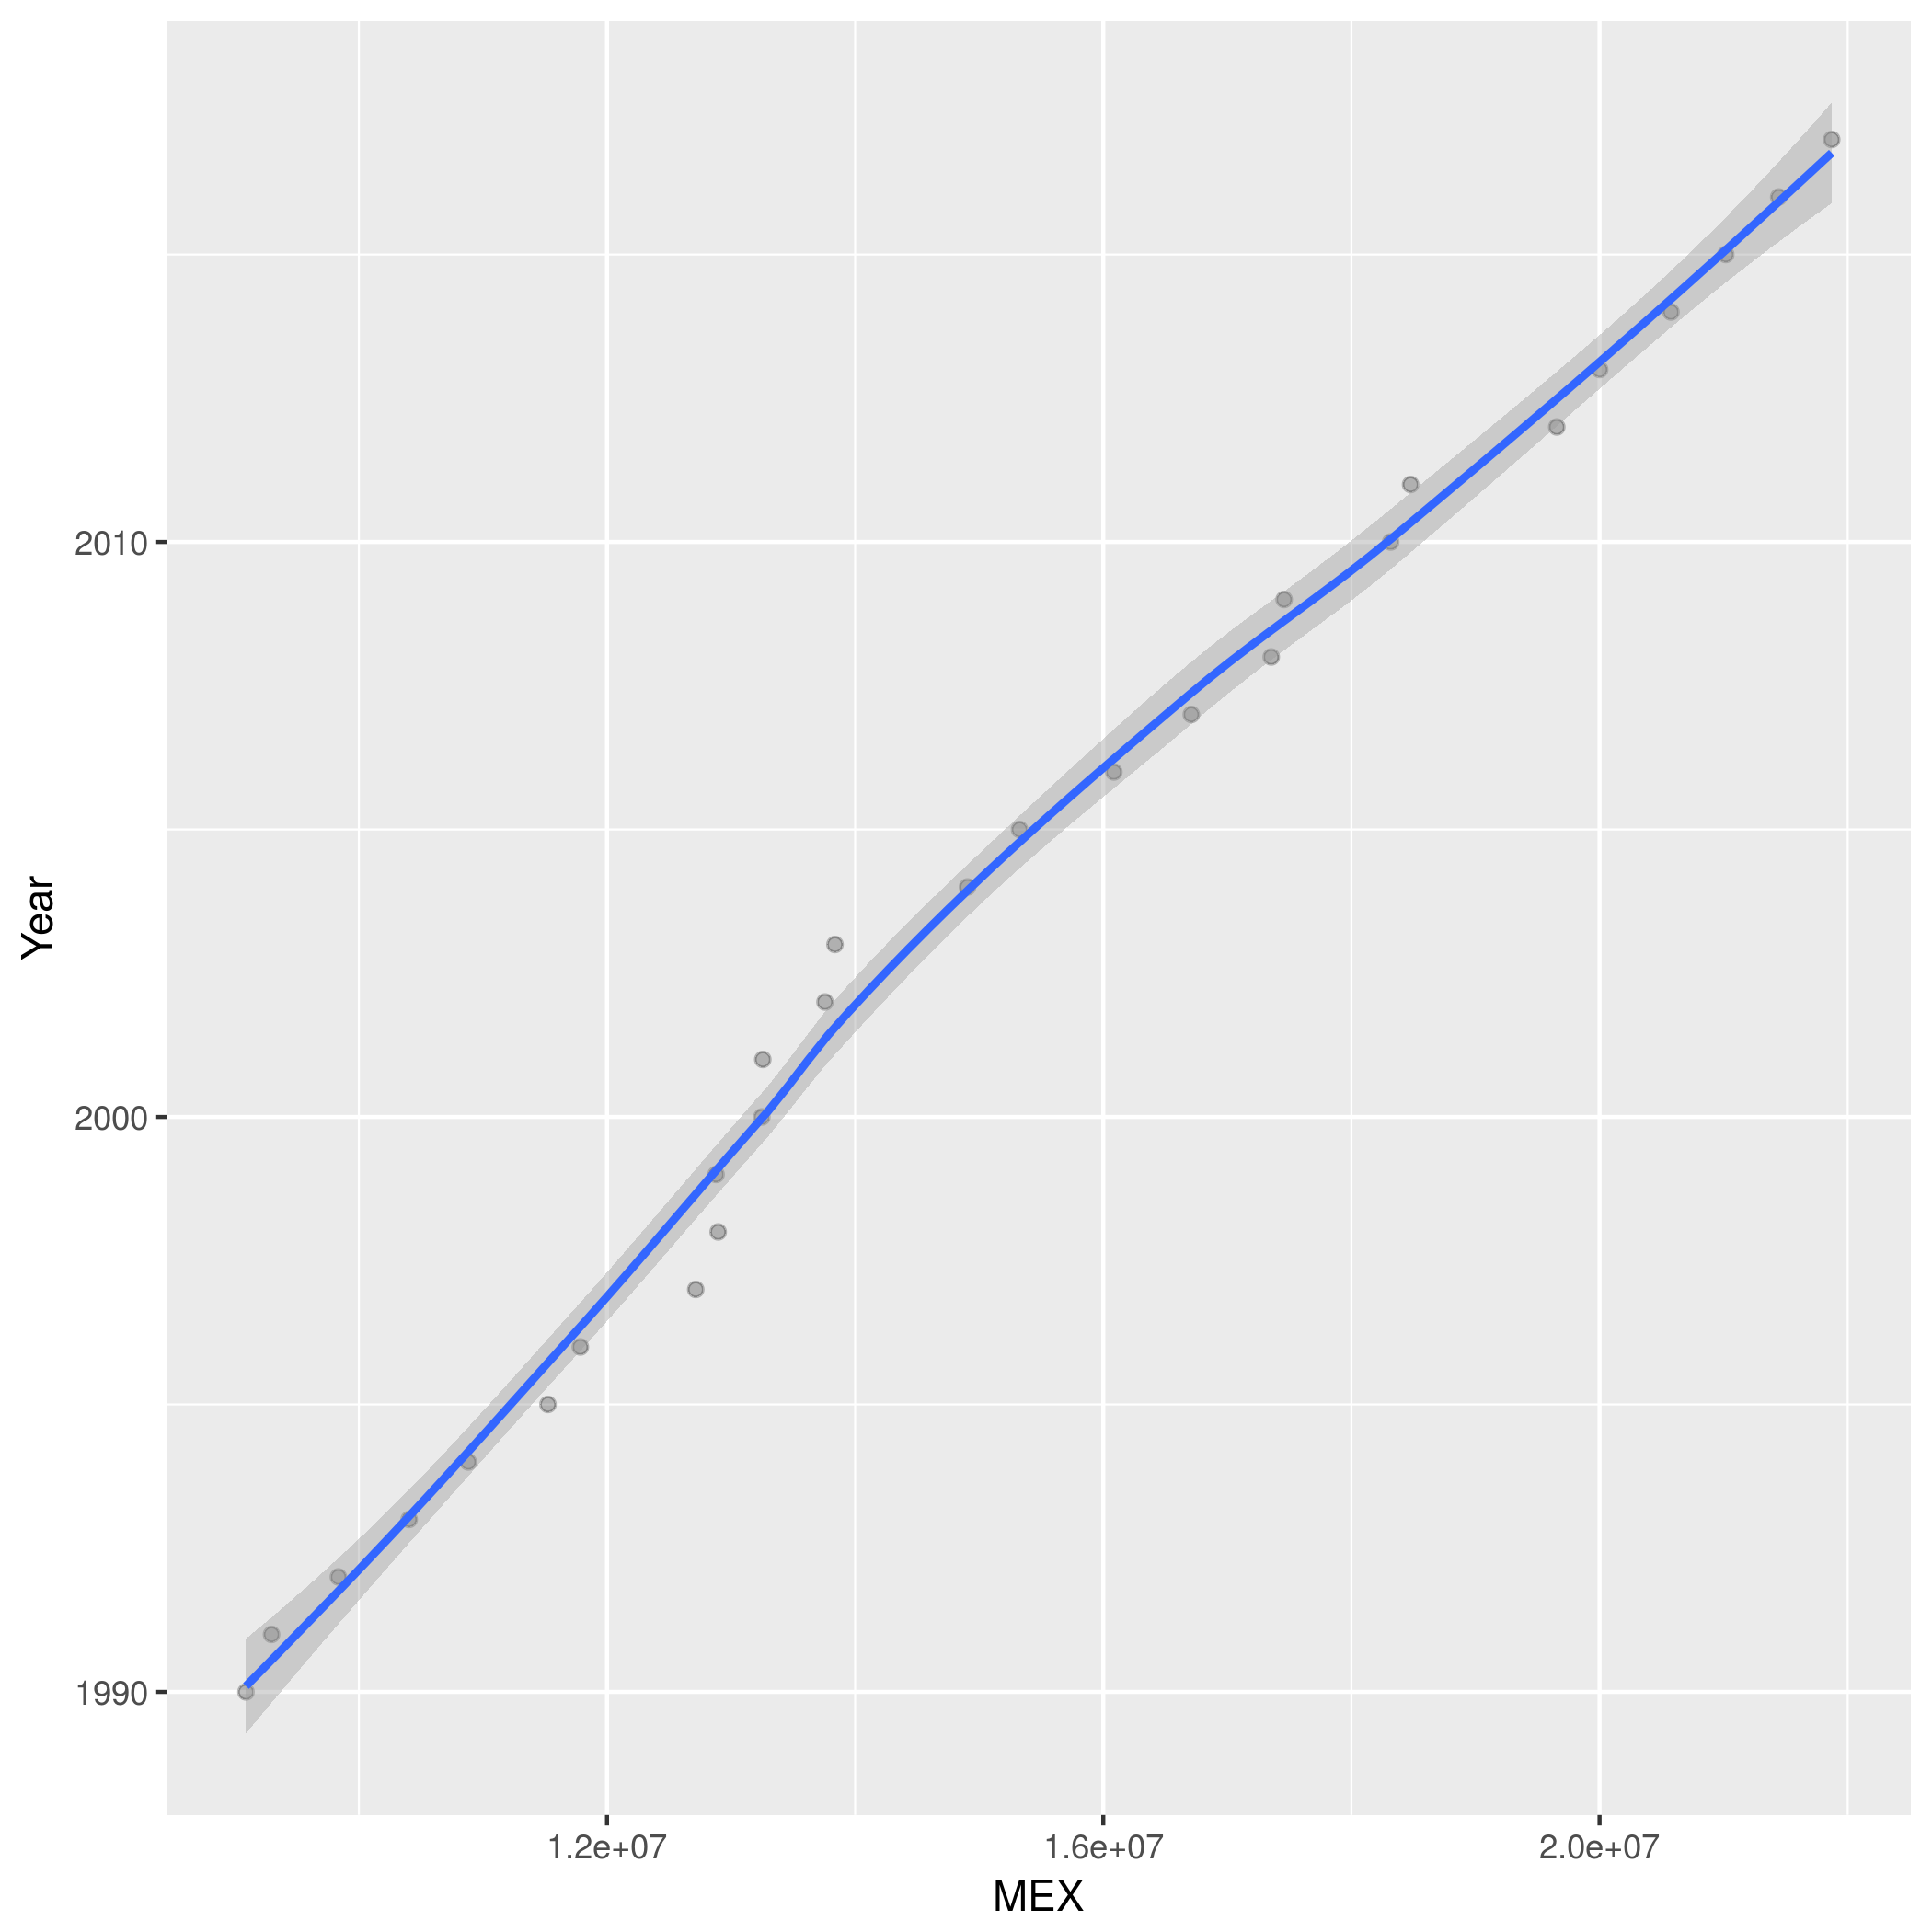
\includegraphics[scale=.5]{quest3Mexico2.png}
\end{figure}

\begin{figure}[h!]
\caption{Increase in women in the labor force for Mexico }
\centering
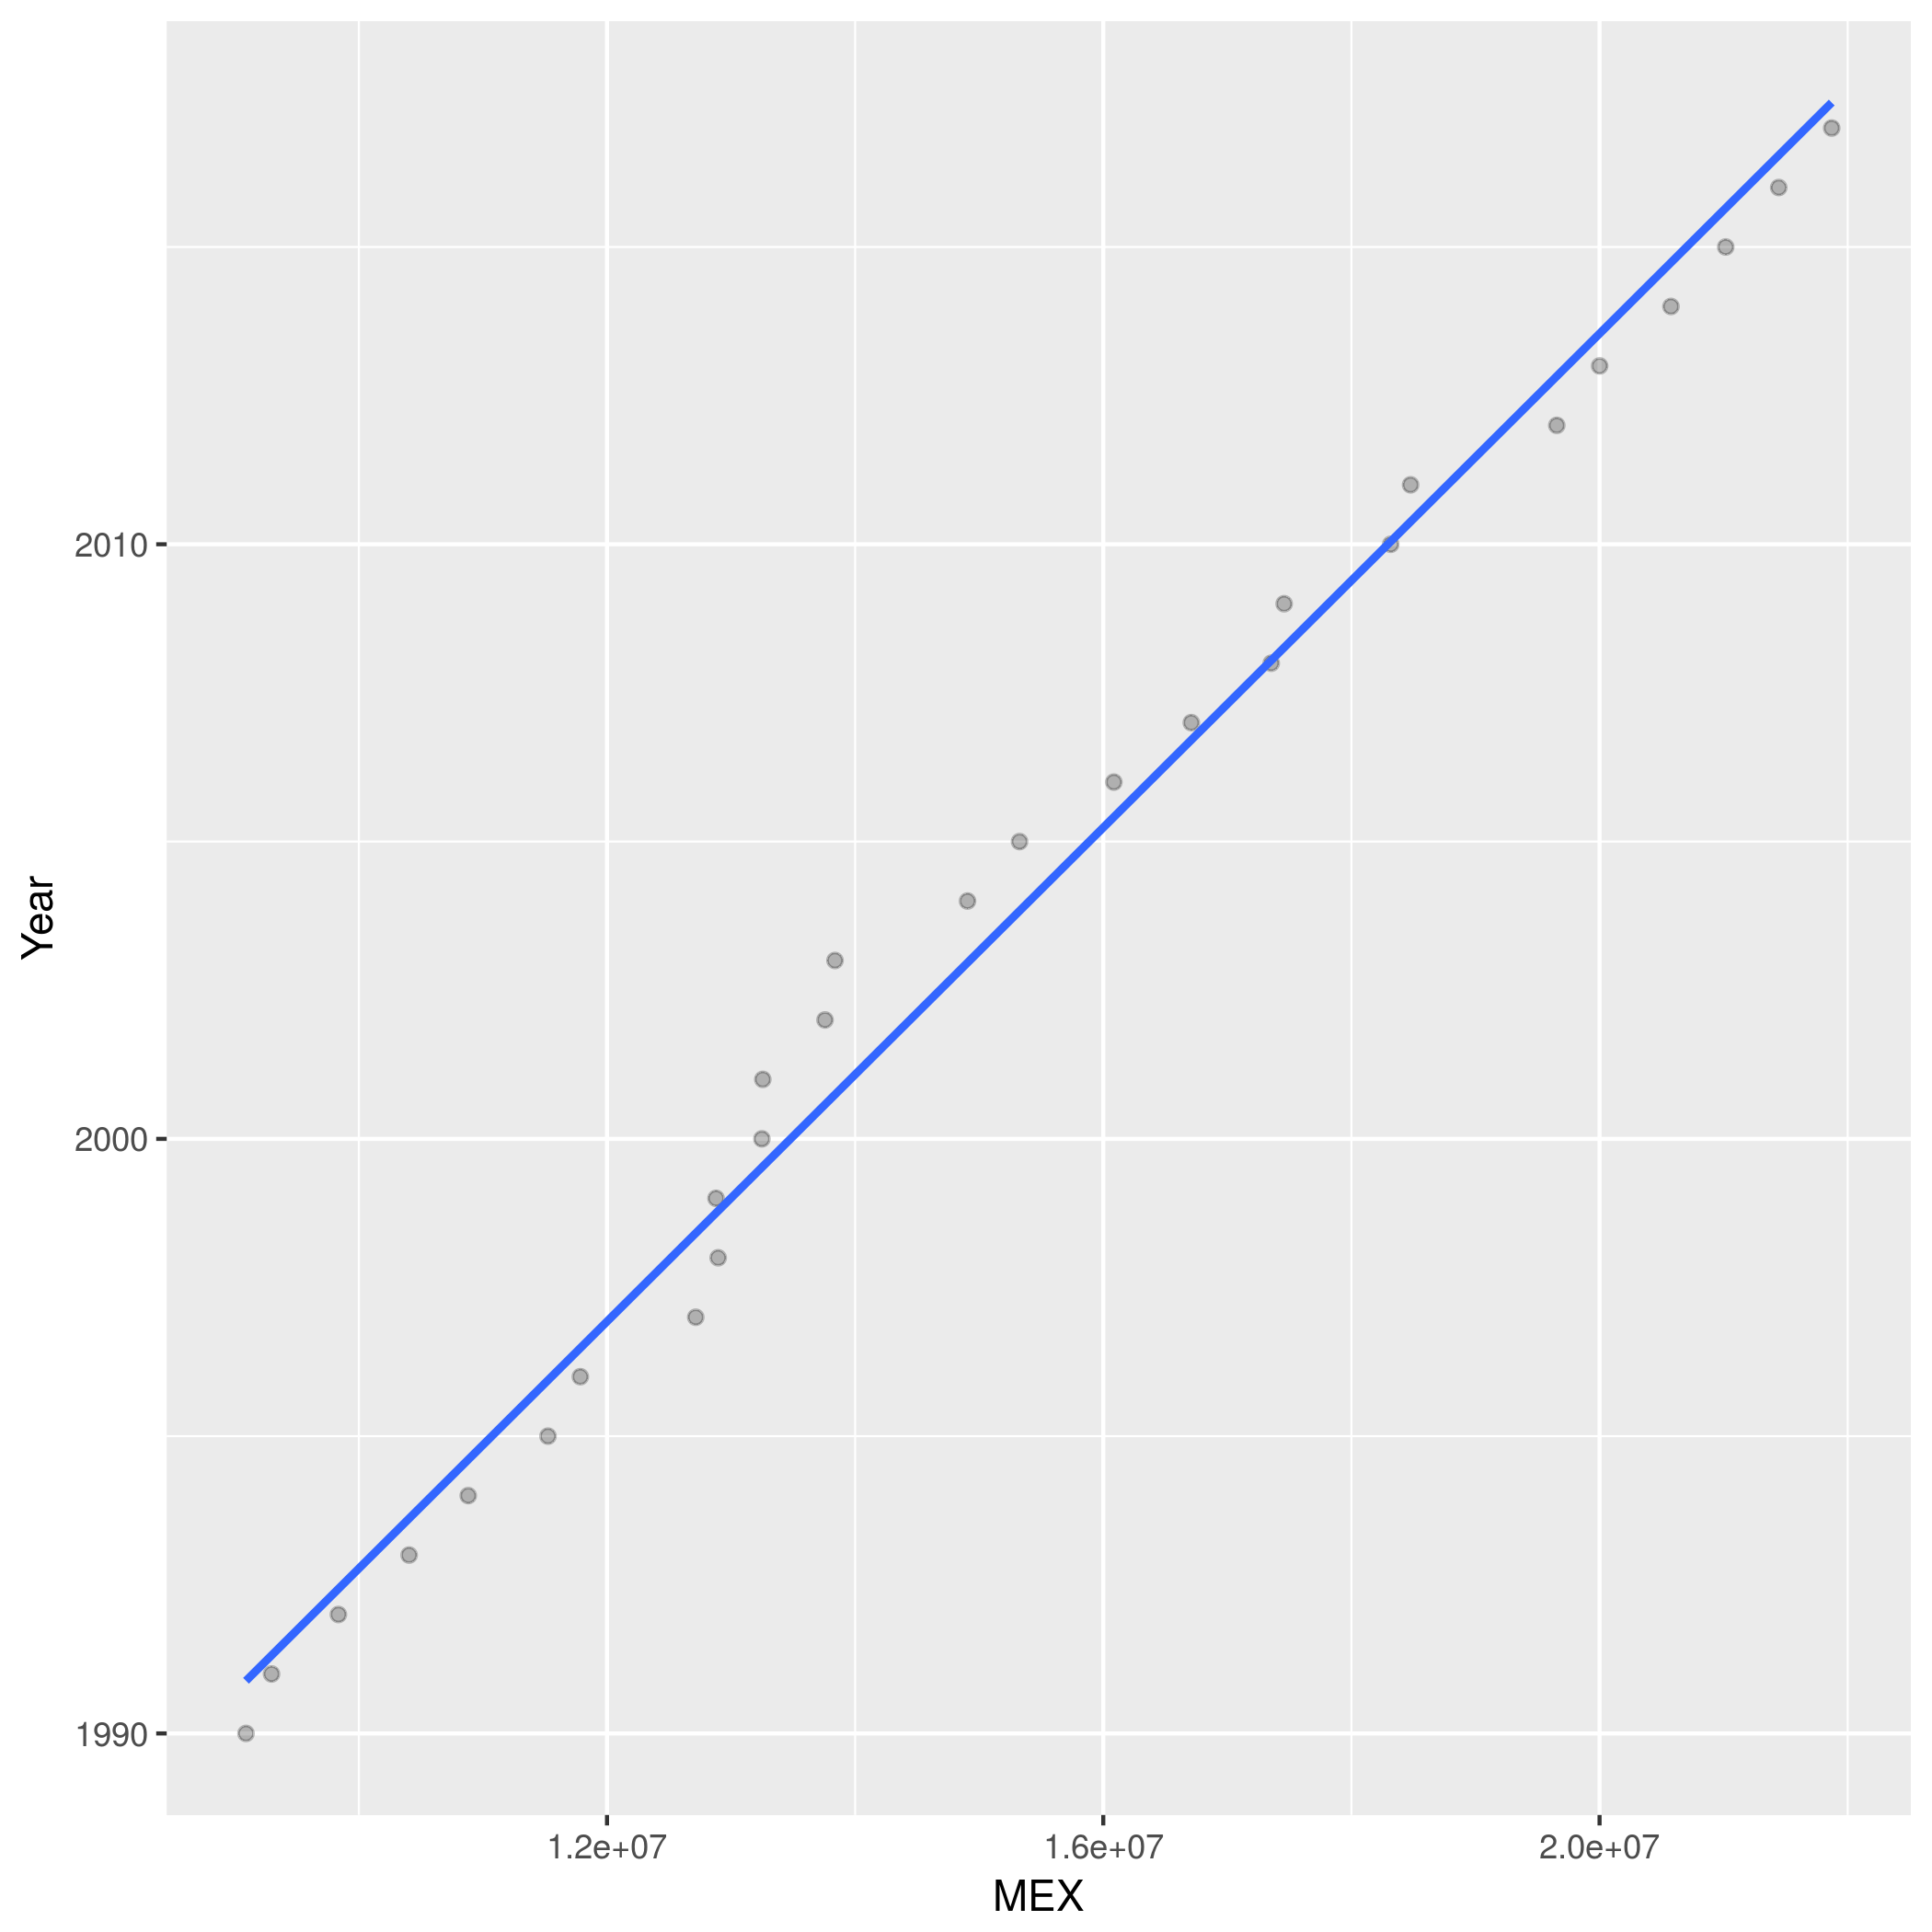
\includegraphics[scale=.5]{quest3Mexico.png}
\end{figure}

\clearpage

\begin{figure}[h!]
\caption{Increase in women in the labor force for USA }
\centering
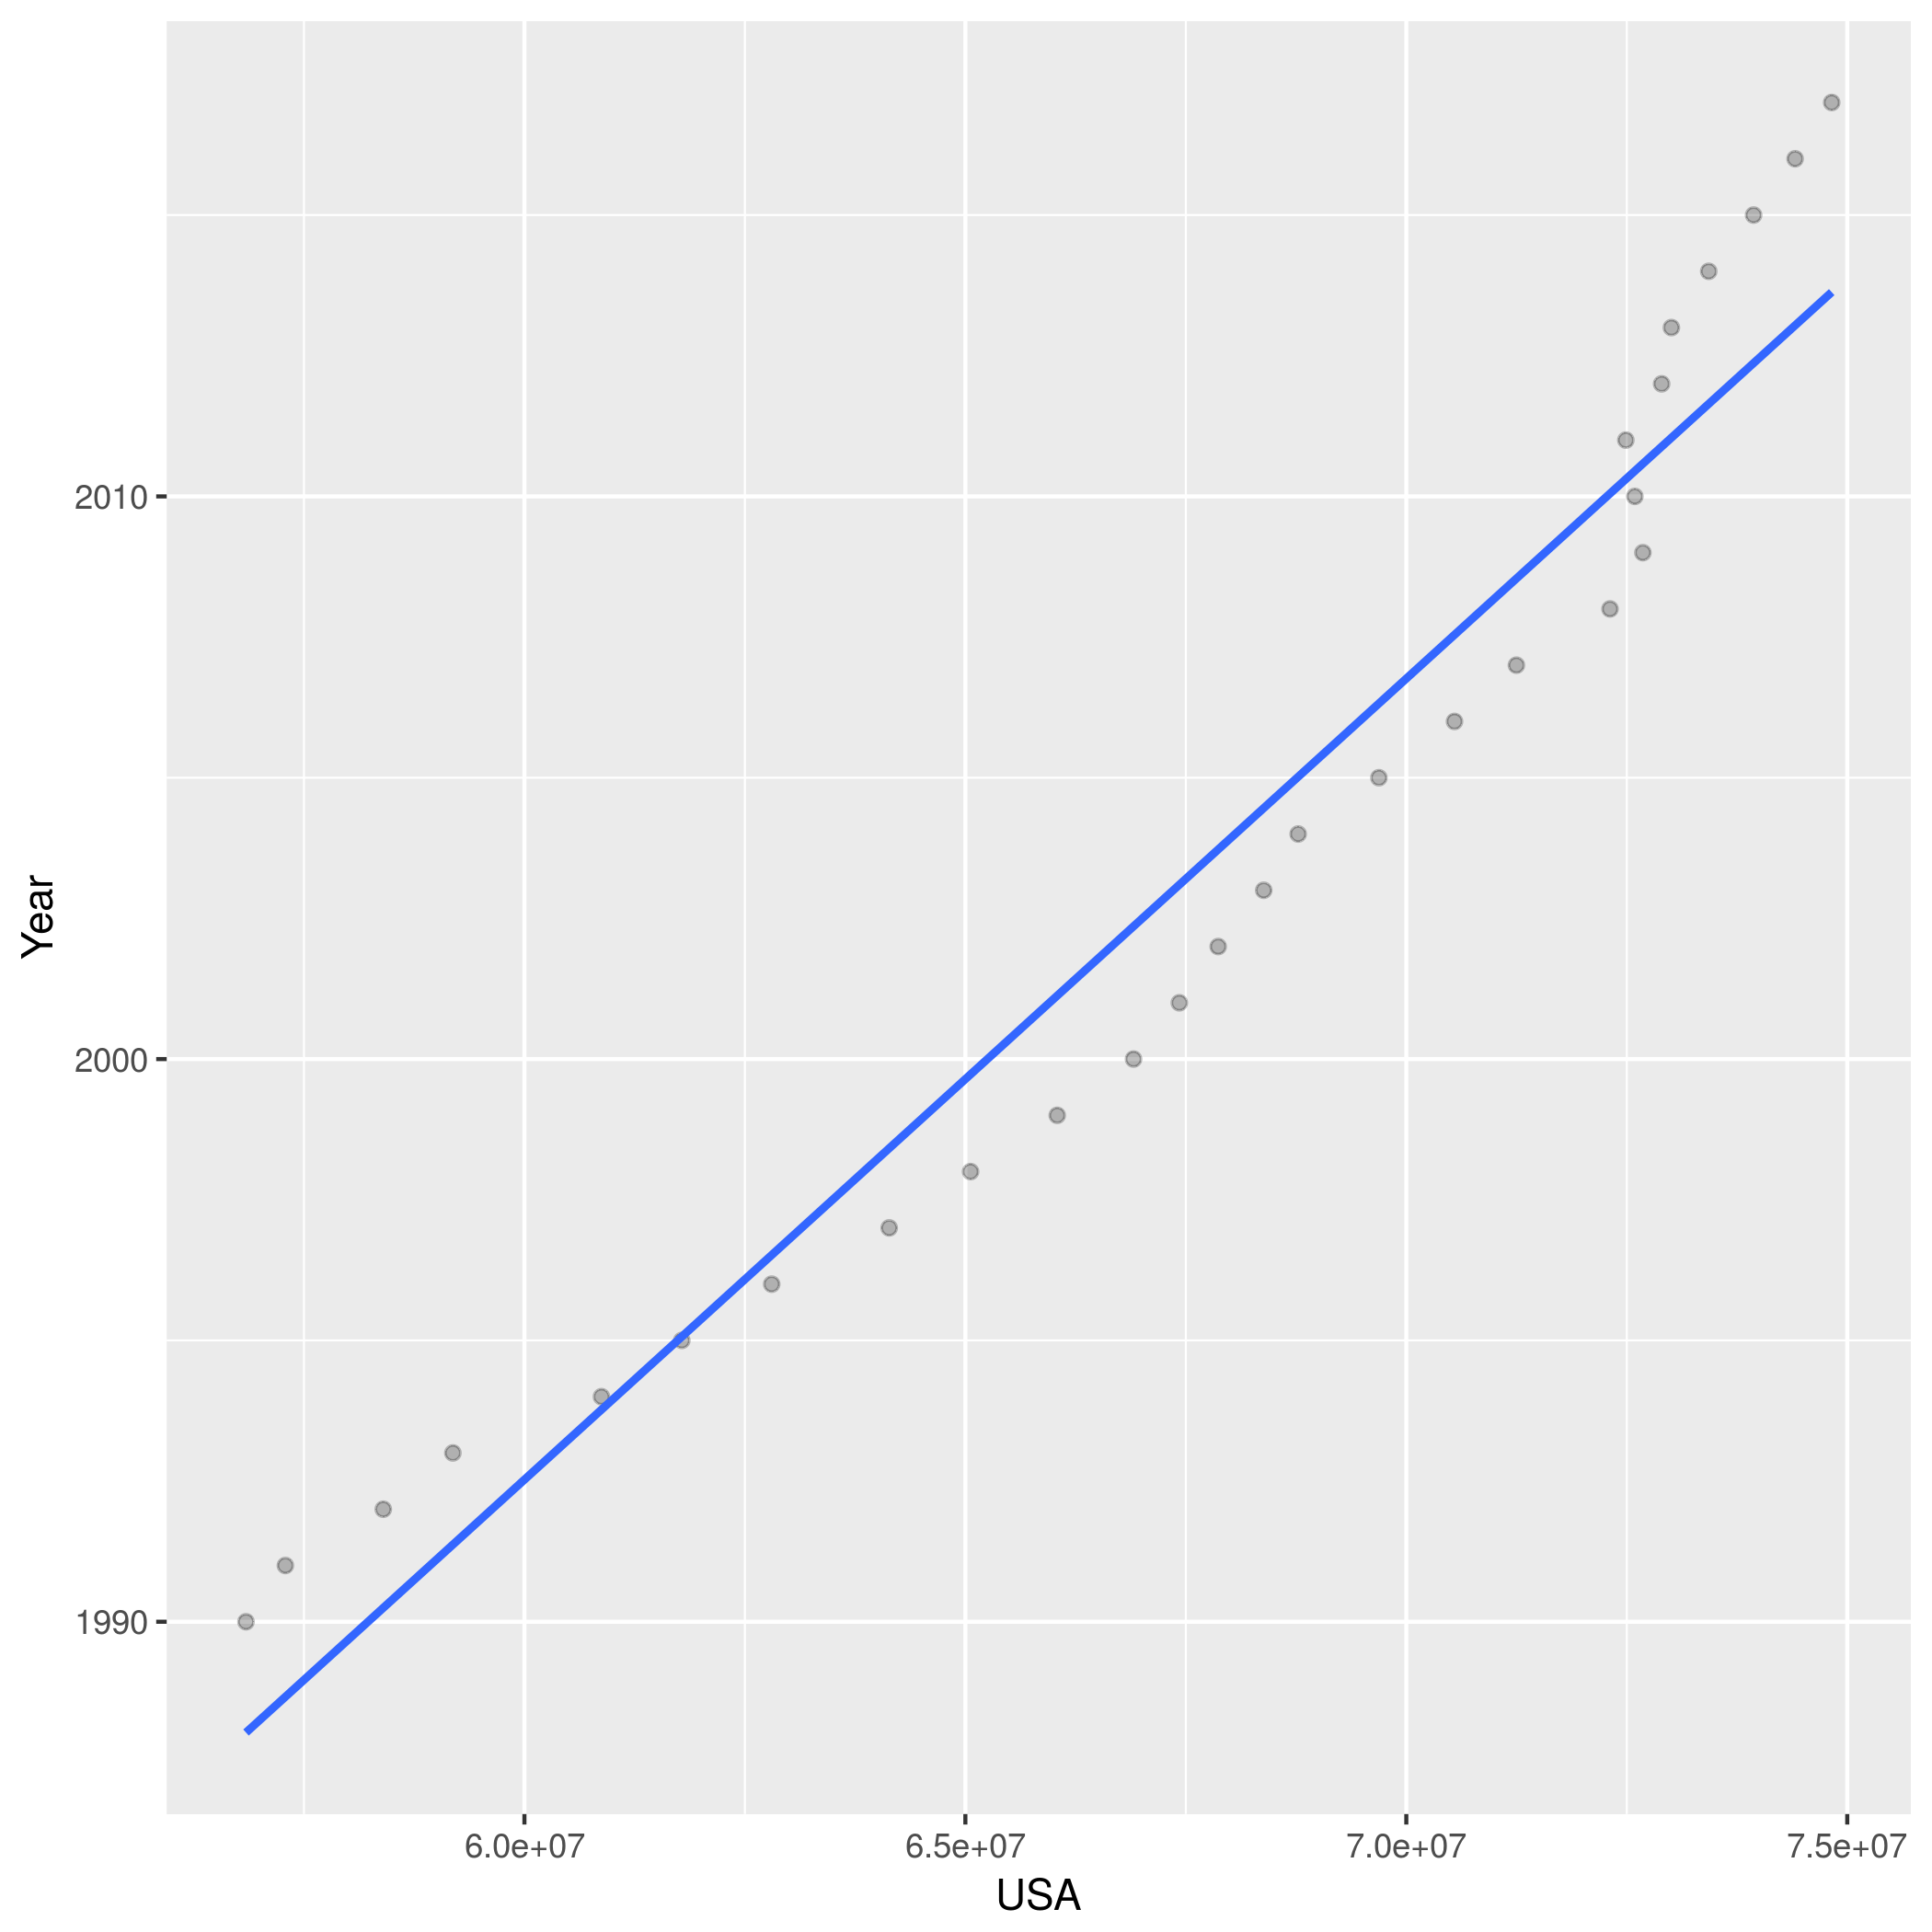
\includegraphics[scale=.5]{quest3USA.png}
\end{figure}
\clearpage

\section{Statement 4: The change in womens bargaining power within the household.}


\begin{figure}[h!]
\caption{Women in decision making about their health Peru}
\centering
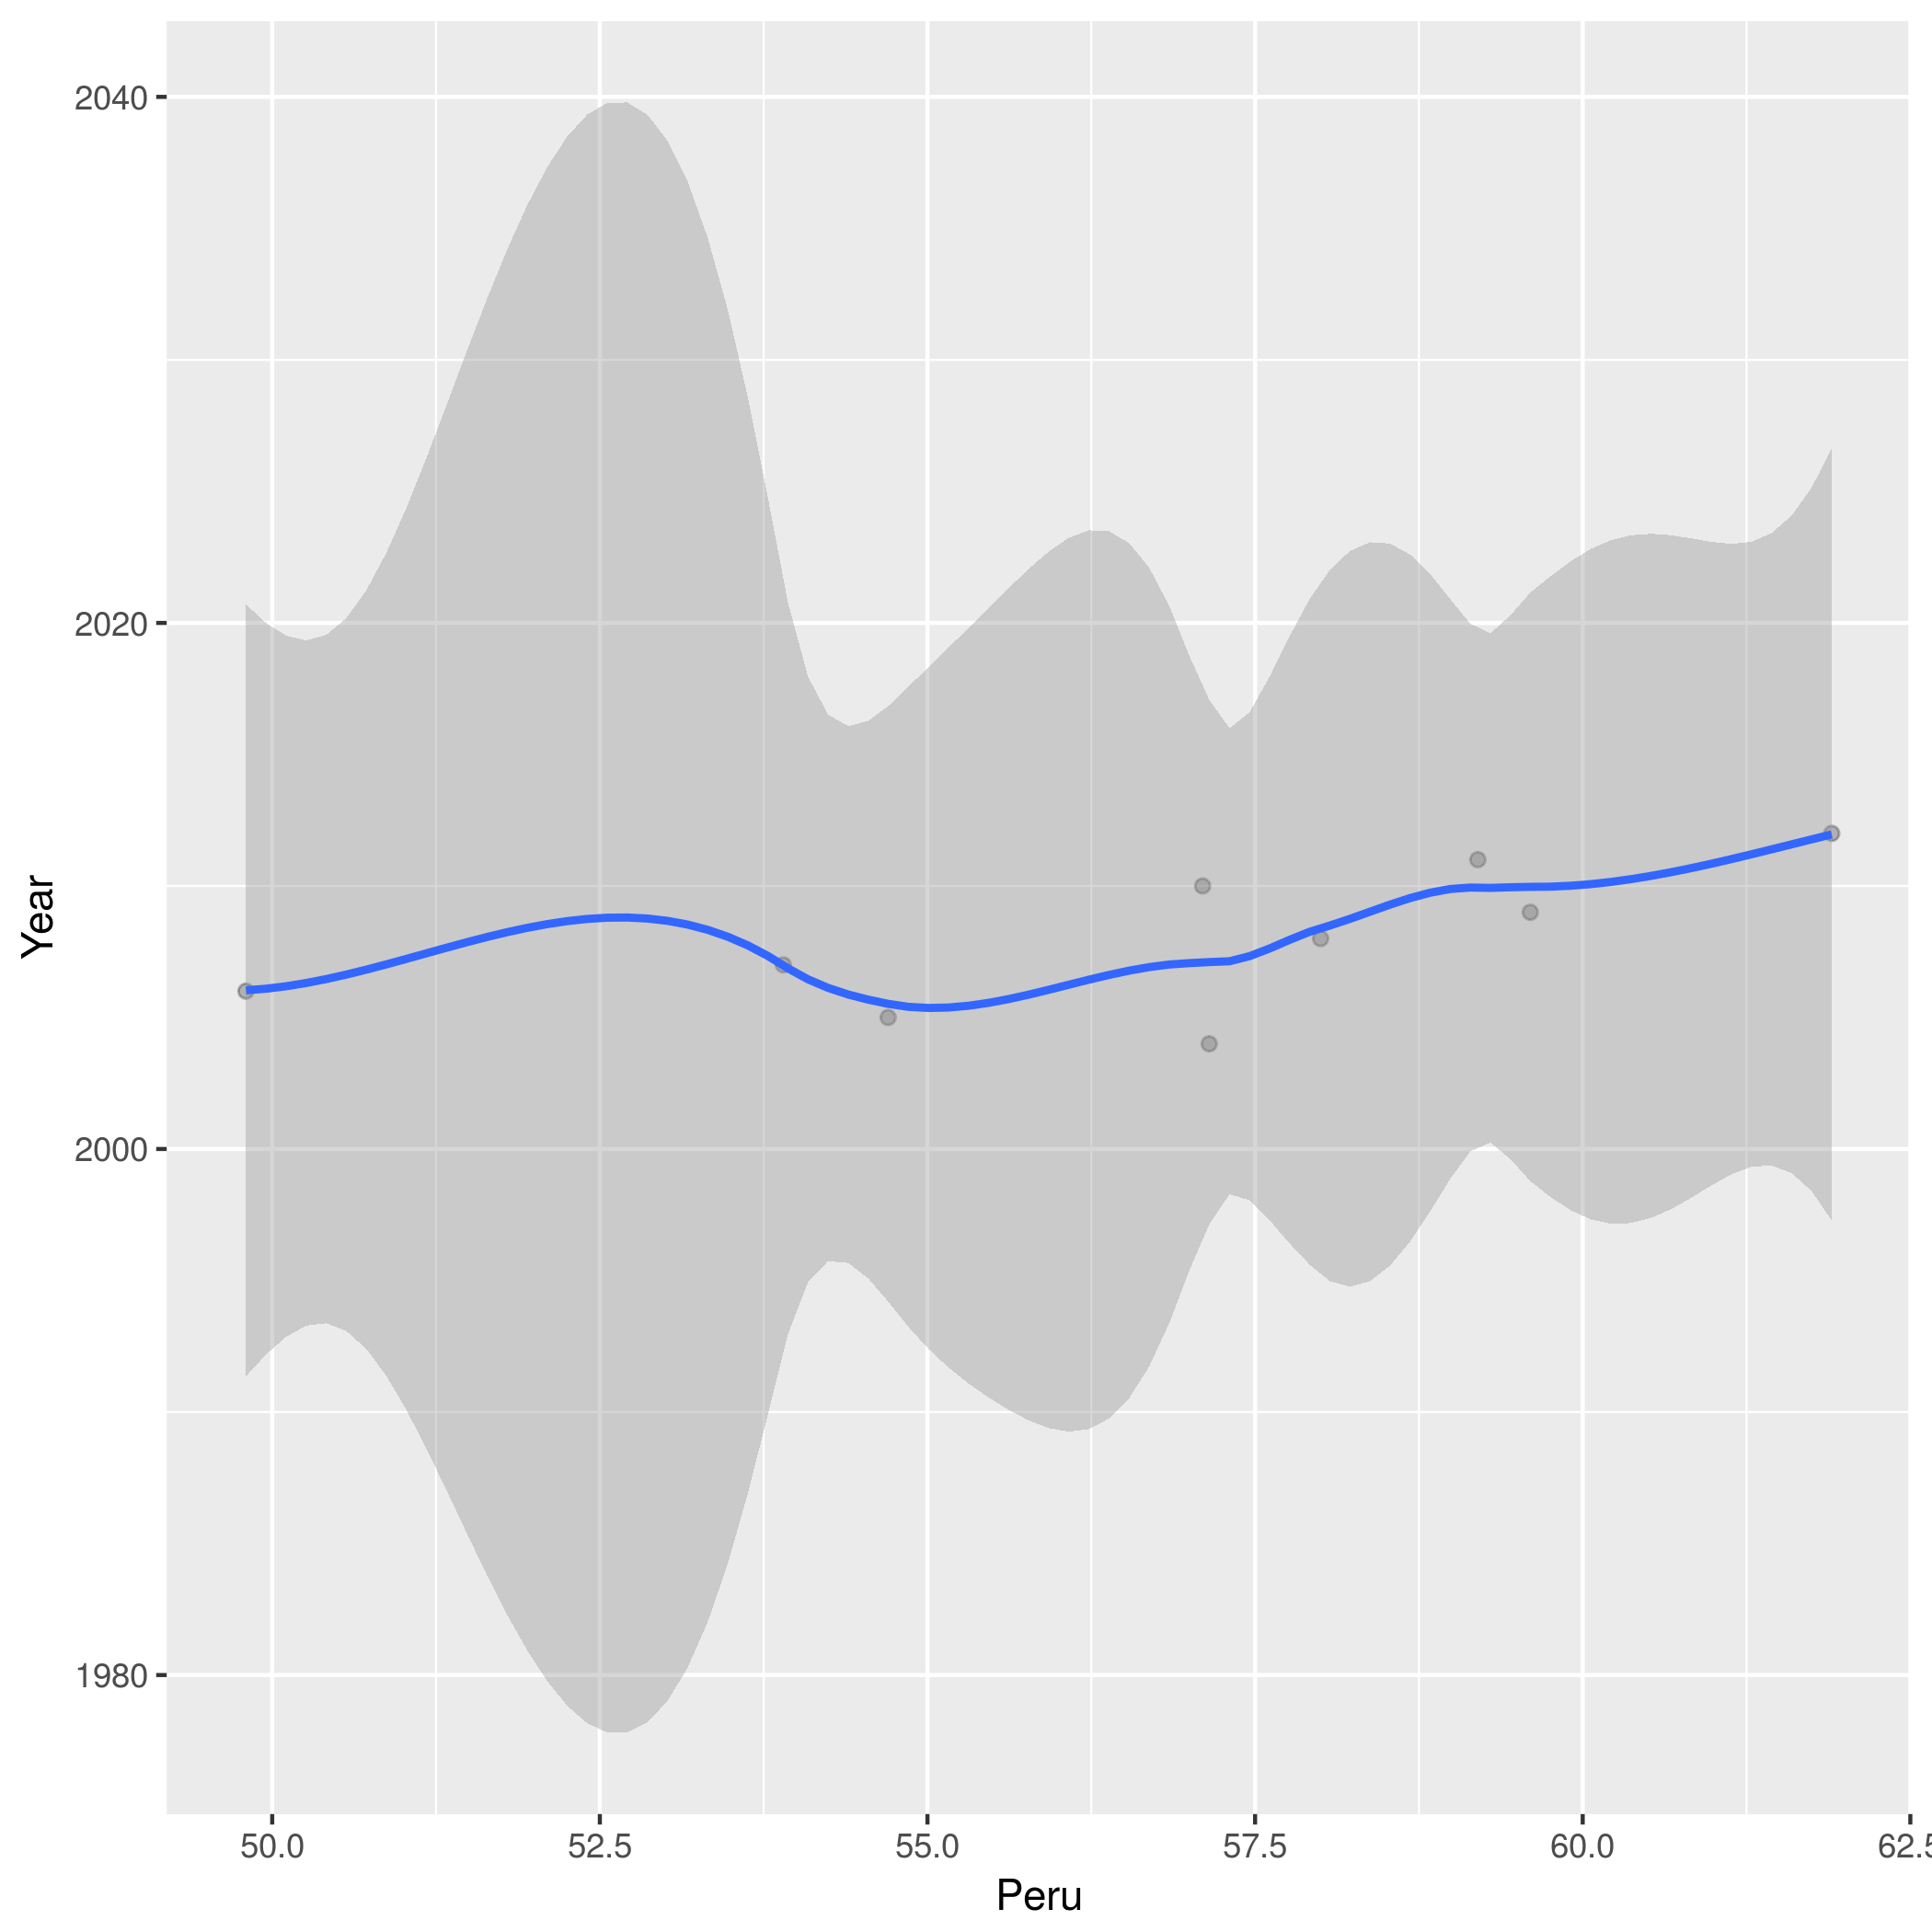
\includegraphics[scale=.5]{quest4Peru.png}
\end{figure}
\clearpage

\begin{figure}[h!]
\caption{Women in decision Making in about their health Bangladesh }
\centering
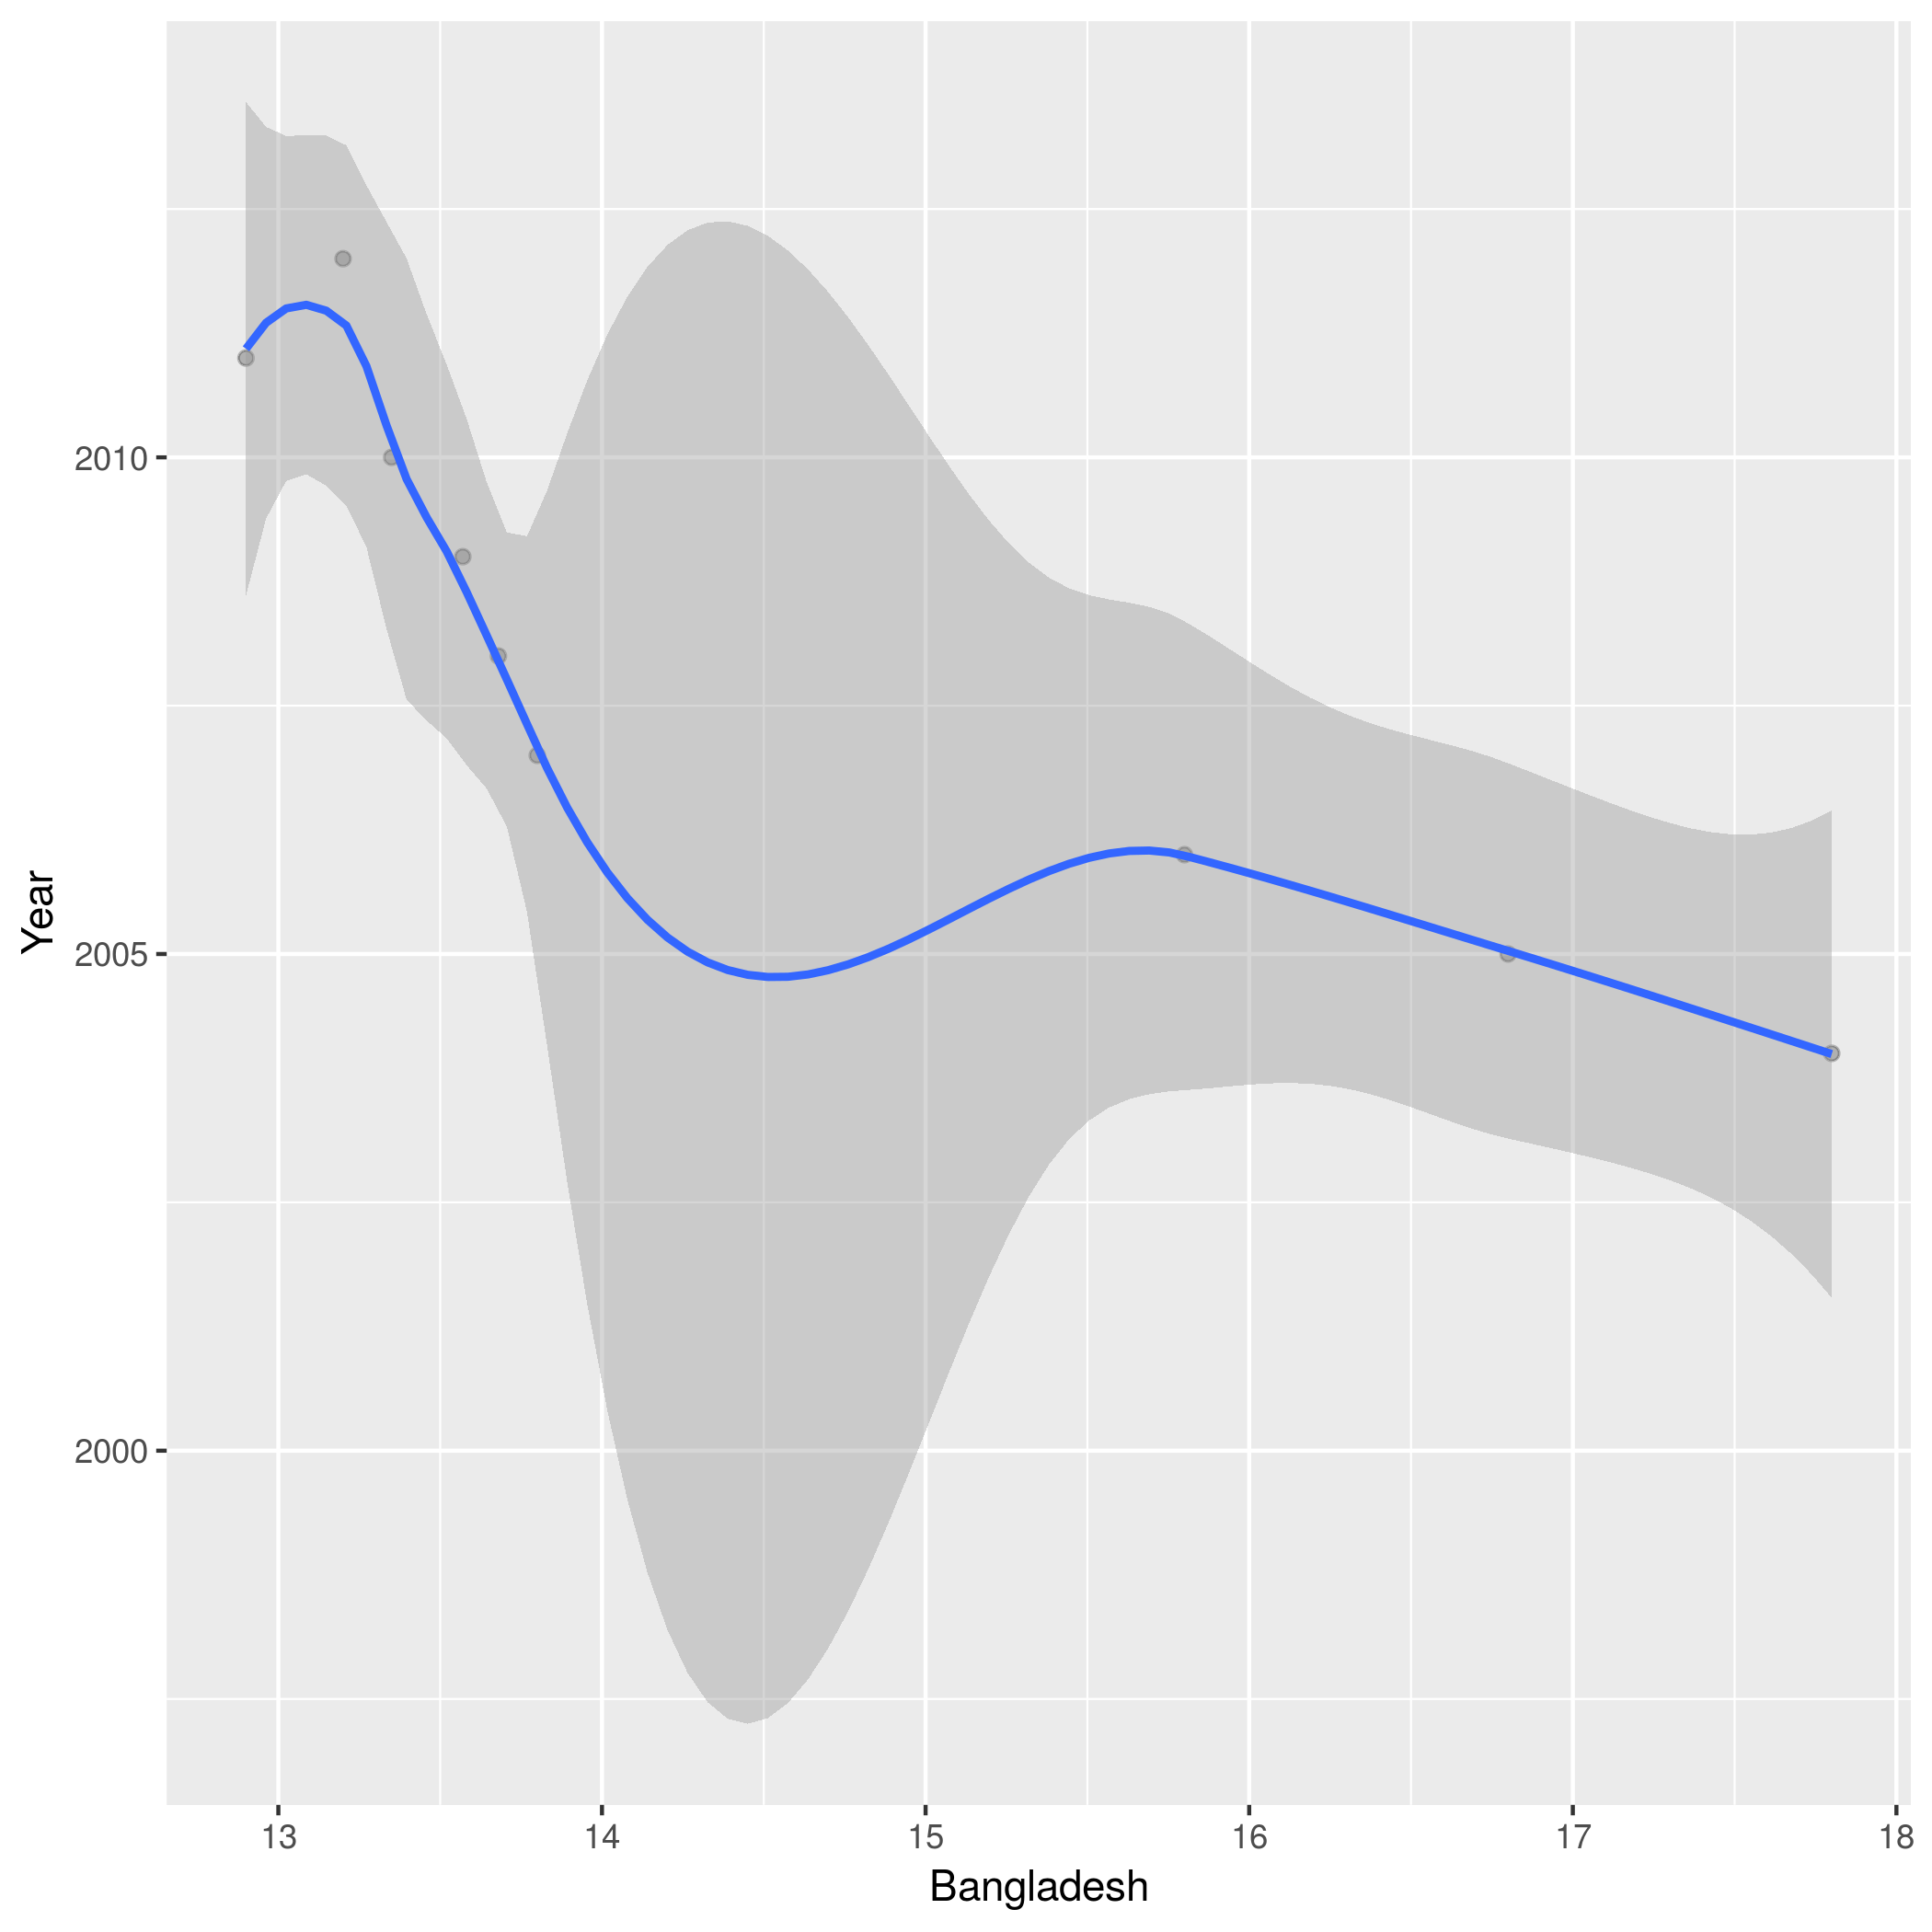
\includegraphics[scale=.5]{quest4Bangladesh.png}
\end{figure}
\clearpage


\begin{figure}[h!]
\caption{Decision making about major household purchase  }
\centering
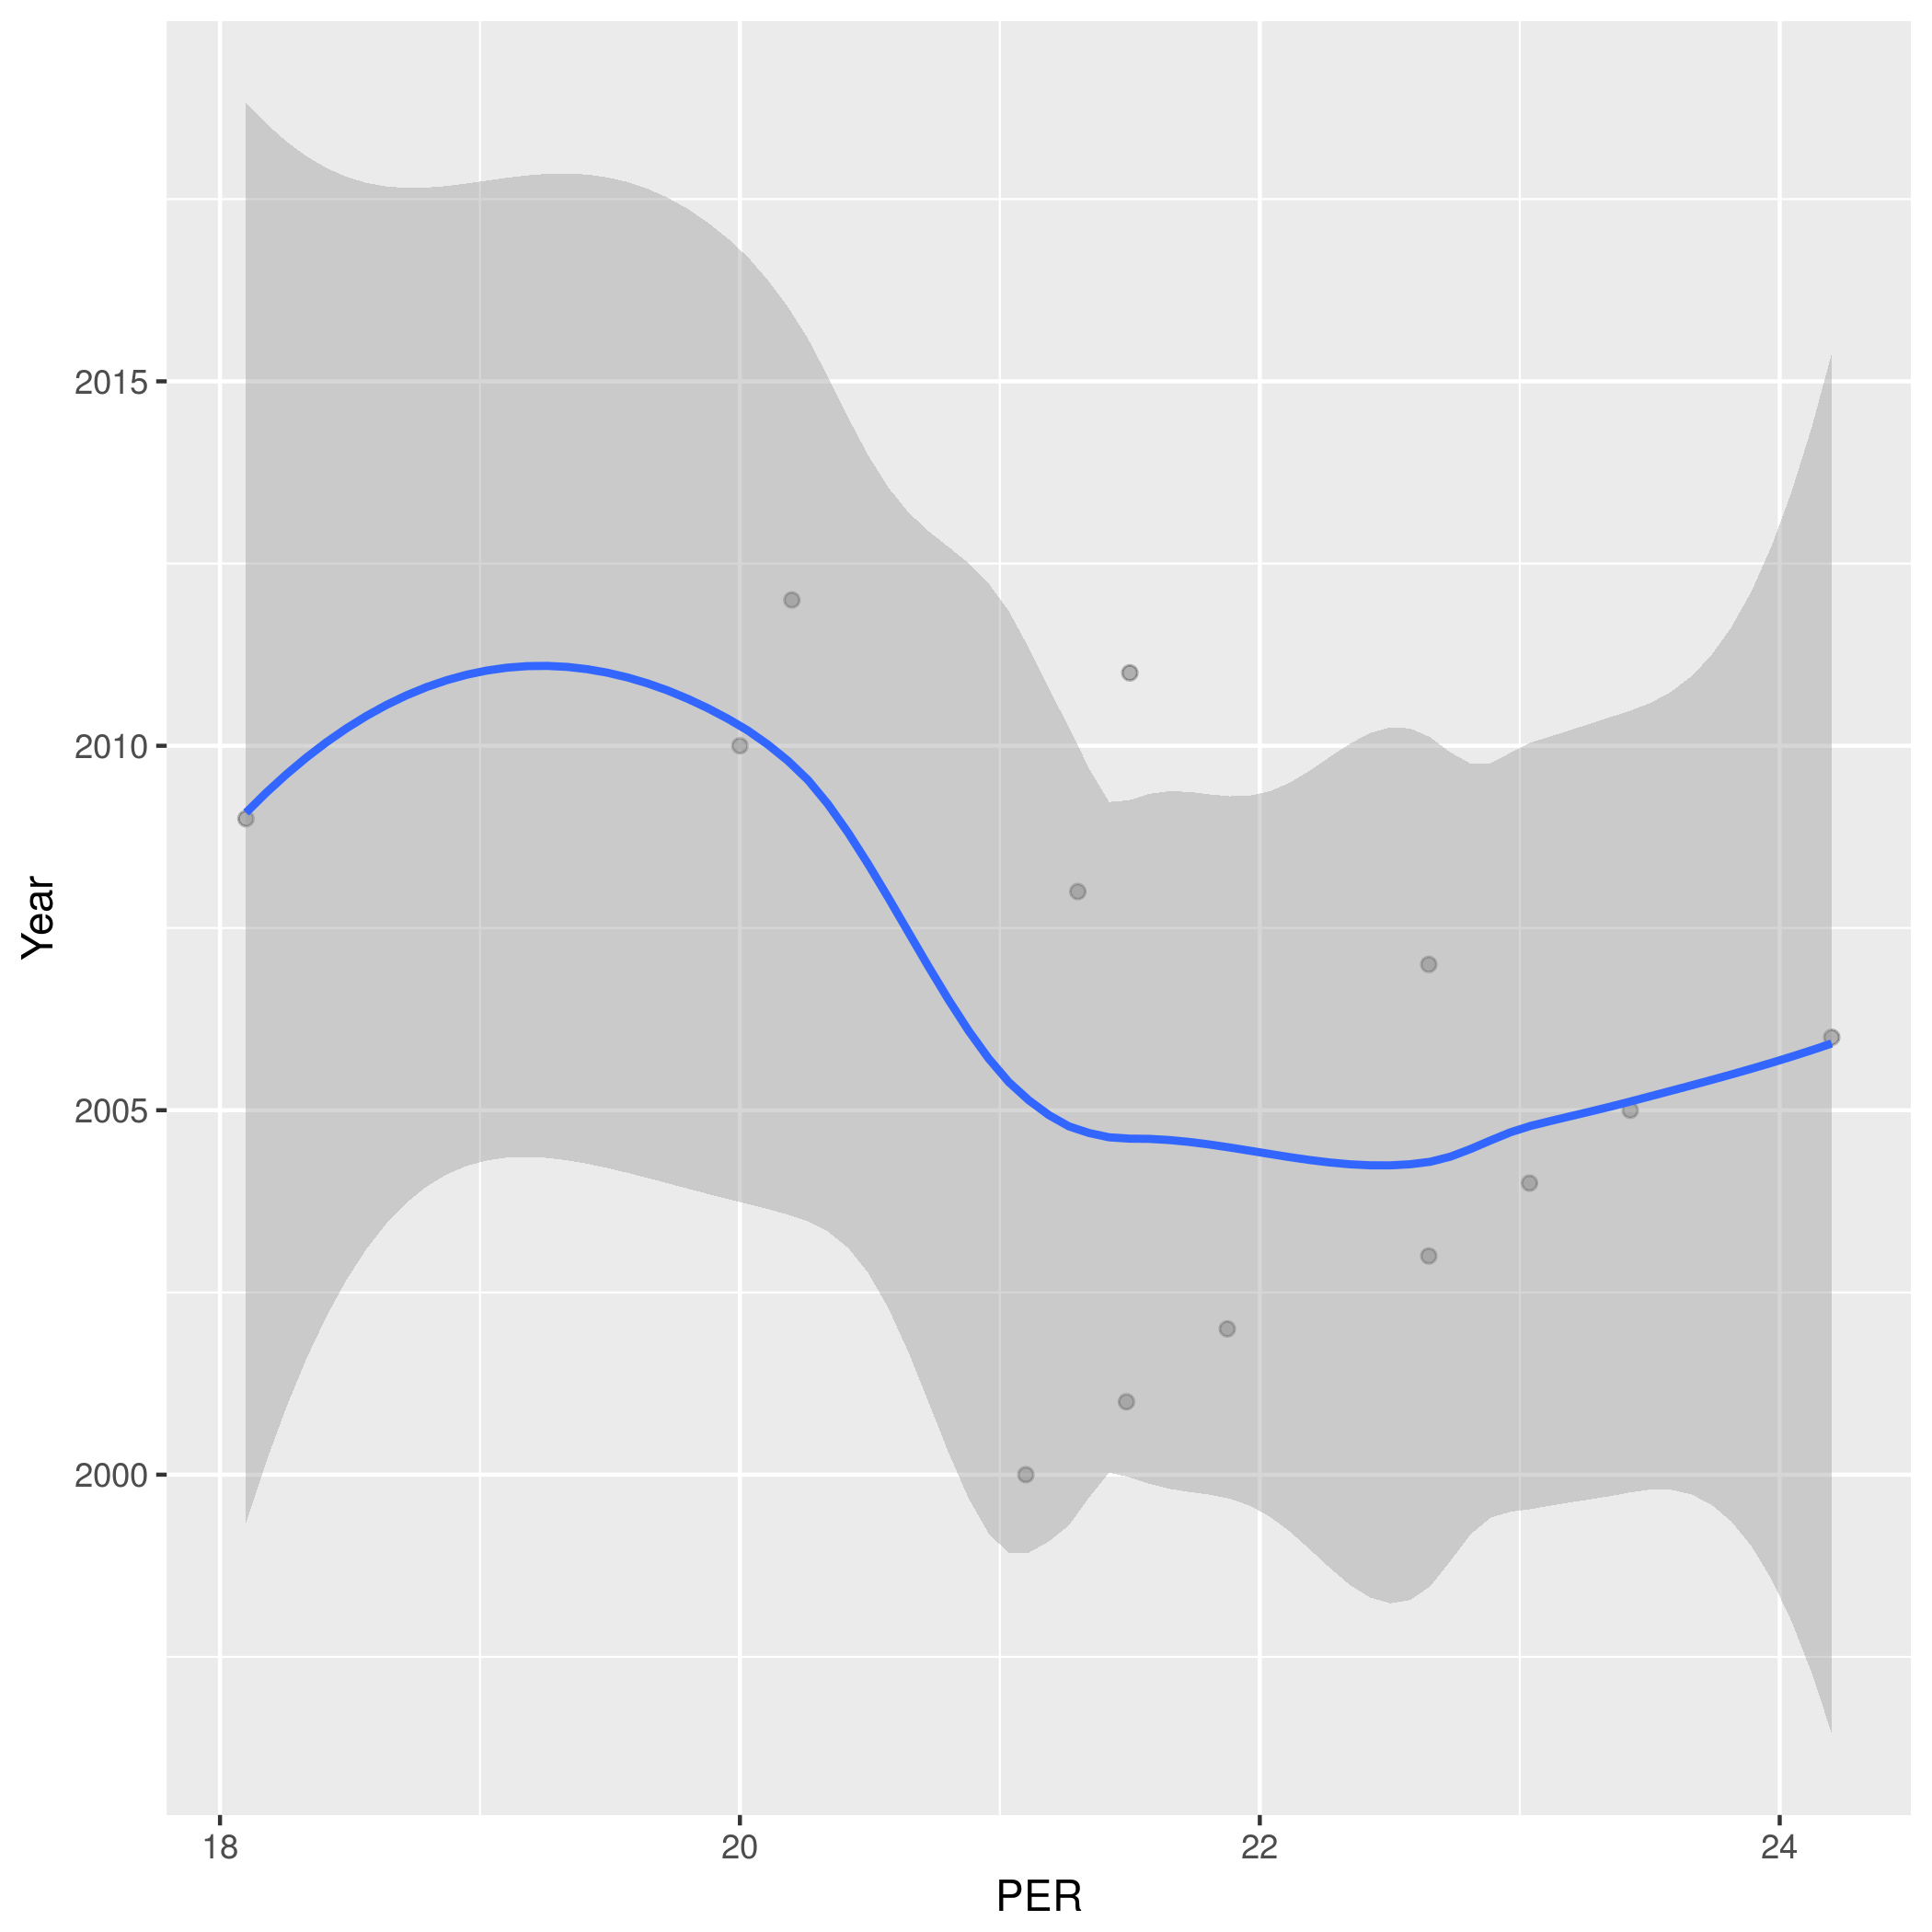
\includegraphics[scale=.5]{quest4Peru2.png}
\end{figure}
\clearpage


\section{Psychology professor  and Econ Professor}

The first thing that I noted that was the biggest difference between Economics and psychology is that the data for economics is concrete, opposed to the psychology data. I mean the Data analyst or data collector has to figure out how much weight an answer would hold when asked a person for an answer. Question have to be manipulated for human error in the sense of asking question that would kind infer to the answer. They both have to make judgment in the amount of data they can collect. Usually the more data the better, but have difficulty collecting the data. In the sense of finding the right sample size to collect their data.





\newpage
\bibliographystyle{plain}
\bibliography{source}

\end{document}




